\documentclass[11pt]{article}
\usepackage[a4paper,margin=2.6cm]{geometry}
% macros.tex -- journal-neutral preamble (Paper 3; adapted from the Paper 2 preamble so that the source can move to a journal class)
\usepackage[T1]{fontenc}
\usepackage[utf8]{inputenc}
\usepackage{lmodern}
\usepackage{amsmath,amssymb,amsthm,mathtools}
\usepackage{bm}
\usepackage{booktabs,array,tabularx}
\usepackage{graphicx}
\usepackage[dvipsnames]{xcolor}
\usepackage{multirow}
\usepackage{caption}
\captionsetup{font=small,labelfont=bf}
\usepackage{enumitem}
\usepackage[numbers,sort&compress]{natbib}
\renewcommand{\bibfont}{\raggedright}% long URLs and hashes: no stretched lines
\usepackage[colorlinks=true,linkcolor=blue!50!black,citecolor=blue!50!black,urlcolor=blue!50!black]{hyperref}
\usepackage[capitalise,noabbrev]{cleveref}
\usepackage{xurl}
\usepackage{seqsplit}
\newcommand{\code}[1]{\nolinkurl{#1}}
\newcommand{\hash}[1]{{\footnotesize\texttt{\seqsplit{#1}}}}

% ---------- theorem environments ----------
\theoremstyle{plain}
\newtheorem{proposition}{Proposition}[section]
\newtheorem{lemma}[proposition]{Lemma}
\newtheorem{corollary}[proposition]{Corollary}
\theoremstyle{definition}
\newtheorem{definition}[proposition]{Definition}
\theoremstyle{remark}
\newtheorem{remark}[proposition]{Remark}
% Named main results (Theorem A, Lemma M, Lemma K, Proposition B1, Lemma Q, Proposition B2, Proposition B3, ...);
% the names are those of the repository, so that every statement can be traced to its proof record.
\newcommand{\resultname}{}
\theoremstyle{plain}
\newtheorem*{namedresultinner}{\resultname}
\newenvironment{named}[1]{\renewcommand{\resultname}{#1}\begin{namedresultinner}}{\end{namedresultinner}}
\crefname{proposition}{Proposition}{Propositions}
\crefname{lemma}{Lemma}{Lemmas}
\crefname{remark}{Remark}{Remarks}
\crefname{table}{Table}{Tables}
\crefname{figure}{Figure}{Figures}
\newcommand{\thmA}{\hyperref[thm:A]{Theorem~A}}
\newcommand{\lemM}{\hyperref[lem:M]{Lemma~M}}
\newcommand{\corM}{\hyperref[cor:M]{Corollary~M}}
\newcommand{\lemK}{\hyperref[lem:K]{Lemma~K}}
\newcommand{\propBone}{\hyperref[prop:B1]{Proposition~B1}}
\newcommand{\lemQ}{\hyperref[lem:Q]{Lemma~Q}}
\newcommand{\propBtwo}{\hyperref[prop:B2]{Proposition~B2}}
\newcommand{\propBthree}{\hyperref[prop:B3]{Proposition~B3}}
\newcommand{\corBthree}{\hyperref[cor:B3]{Corollary~B3$'$}}

% ---------- author notes and release placeholders (set \draftnotesfalse to hide author notes) ----------
\newif\ifdraftnotes \draftnotestrue
\newcommand{\authornote}[1]{\ifdraftnotes{\color{BrickRed}\textsf{[#1]}}\fi}
% Release placeholders: always visible, easy to locate (search for "TO BE ASSIGNED AT PUBLIC RELEASE").
\newcommand{\PaperThreeGitHub}{{\color{BrickRed}\textsf{[PAPER 3 GITHUB RELEASE --- TO BE ASSIGNED AT PUBLIC RELEASE]}}}
\newcommand{\PaperThreeDOI}{{\color{BrickRed}\textsf{[PAPER 3 ZENODO DOI --- TO BE ASSIGNED AT PUBLIC RELEASE]}}}

% ---------- notation ----------
\newcommand{\R}{\mathbb{R}}
\newcommand{\Z}{\mathbb{Z}}
\newcommand{\ind}{\operatorname{ind}}
\newcommand{\nul}{\operatorname{null}}
\newcommand{\In}{\operatorname{In}}
\newcommand{\tr}{\operatorname{tr}}
\newcommand{\adj}{\operatorname{adj}}
\newcommand{\Fix}{\operatorname{Fix}}
\newcommand{\Stab}{\operatorname{Stab}}
\newcommand{\Span}{\operatorname{span}}
\newcommand{\Vred}{V_{\mathrm{red}}}
\newcommand{\ystar}{y^{*}}
\newcommand{\rstar}{r_{*}}
\newcommand{\qc}{q_{c}}
\newcommand{\Dt}{\widetilde{D}}
\newcommand{\one}{\mathbf{1}}
\newcommand{\eA}{e_{A}}
\newcommand{\ebr}{e_{\mathrm{br}}}
\newcommand{\Ahat}{\widehat{A}}
\newcommand{\Ehat}{\widehat{E}}
\newcommand{\uh}{\widehat{u}}
\newcommand{\vh}{\widehat{v}}
\newcommand{\khat}{\widehat{\kappa}}
\newcommand{\cfhat}{\widehat{c}_4}
\newcommand{\Mhat}{\widehat{M}}
\newcommand{\Aonegg}{A_{1g}}
\newcommand{\Eg}{E_{g}}
\newcommand{\Tonegg}{T_{1g}}
\newcommand{\Ttwog}{T_{2g}}
\newcommand{\Atwou}{A_{2u}}
\newcommand{\Eu}{E_{u}}
\newcommand{\Toneu}{T_{1u}}
\newcommand{\Ttwou}{T_{2u}}
\newcommand{\Oh}{O_{h}}
\newcommand{\Td}{T_{d}}
\newcommand{\Dthreed}{D_{3d}}
\newcommand{\Dtwoh}{D_{2h}}
\newcommand{\Dfourh}{D_{4h}}
\newcommand{\repo}{\code{EIT_LJ_CUBE_BIFURCATIONS}}

\hypersetup{pdftitle={Symmetry-Breaking Bifurcations from the Cubic Equilibrium in Two-Term Inverse-Power Clusters},
  pdfauthor={Toni Mladenovski; Mihail Mladenski}}

\title{Symmetry-Breaking Bifurcations from the Cubic Equilibrium\\ in Two-Term Inverse-Power Clusters}
\author{Toni Mladenovski$^{1,*}$\quad$\cdot$\quad Mihail Mladenski$^{1}$}
\date{\small $^{1}$EITNetworks LLC, Tobyhanna, Pennsylvania, USA\\[2pt]
$^{*}$Corresponding author: Toni Mladenovski, \texttt{info@eitnetworks.org}, ORCID
\href{https://orcid.org/0009-0009-8343-662X}{0009-0009-8343-662X}\\[6pt]
Version 1.0.0; mathematics as audited at repository version V0.4-dev.6}

\begin{document}
\maketitle

\begin{abstract}
Eight identical particles interacting through the two-term pair potential $\phi(r)=Ar^{-p}-Br^{-q}$ ($A,B>0$,
$p>q>0$) have a cubic equilibrium for every exponent pair. A companion work classified its linear spectrum and showed
that zero modes beyond the six rigid motions occur only on two transition curves: $p=P_A(q)$, where a one-dimensional
$\Atwou$ mode becomes critical, and $p=P_T(q)$, where a three-dimensional $\Ttwog$ mode becomes critical. We determine
the nonlinear local branches born at these curves. On the $\Atwou$ curve the bifurcation is a $\Z_2$-symmetric
pitchfork, supercritical in the reduced-energy convention, whose branches consist of two concentric regular tetrahedra
of unequal radii with point group $\Td$. On the $\Ttwog$ curve the critical representation carries the cubic invariant
$a_1a_2a_3$ with a coefficient that is nonzero along the whole curve; the $\Dthreed$ branches are therefore
transcritical. The $\Dtwoh$ branches are $\Z_2$-symmetric pitchforks, supercritical in the reduced-energy axial
convention, opening towards $p>P_T(q)$; their configurations have point group exactly $\Dtwoh$ and are not cuboids. On
these branches the Hessian of the reduced potential on the three-dimensional centre space has inertia $(1,0,2)$, and
with the frozen spectral data of the companion work the full Hessian modulo rigid motions has inertia $(4,0,14)$:
the branch points are saddles with four unstable directions. The signs of the two nonlinear coefficients that decide
the branch types are proved with rigorous ball-arithmetic certificates; every computer-assisted step, including an
implementation erratum that was found, corrected and closed, was reproduced in independent blind computational audits.
\end{abstract}

\medskip
\noindent\textbf{Keywords:} two-term power-law potential; Lennard-Jones and Mie clusters; equivariant bifurcation;
Lyapunov--Schmidt reduction; octahedral symmetry; Morse index; computer-assisted proof; ball arithmetic.

\noindent\textbf{MSC 2020:} Primary 37G40, 70F10; Secondary 58K05, 20C35, 65G20.

\tableofcontents

\section{Introduction}\label{sec:intro}

Small clusters bound by pair potentials are a classical object of mathematical chemistry: their equilibria,
saddles and rearrangement pathways organise the energy landscape
\citep{HoarePal1971,HoareMcInnes1983,DoyeWales2002,Trombach2018,SchwerdtfegerWales2024}. For the two-term family
\begin{equation}\label{eq:pot}
\phi(r)=Ar^{-p}-Br^{-q},\qquad A,B>0,\quad p>q>0,
\end{equation}
which contains the Lennard-Jones potential $(p,q)=(12,6)$ and the Mie potentials, symmetric configurations are
equilibria for structural reasons, and their stability can change with the exponents. The eight-particle cube is the
simplest such configuration with a nontrivial spectrum.

A companion work \citep{Paper2} (``Paper~2'') settled the linear problem. With the exact $\Oh$ block decomposition of
the $24$-dimensional displacement space it showed that the cubic equilibrium is a saddle for every $p>q>0$, with Morse
index $2+\one\{q\ge\rstar\text{ or }p>P_A(q)\}+3\cdot\one\{q\ge\qc\text{ or }p>P_T(q)\}\in\{2,3,6\}$, and that zero
modes other than the six rigid motions occur exactly on two disjoint transition curves: $p=P_A(q)$ ($0<q<\rstar$),
where a one-dimensional $\Atwou$ eigenvalue changes sign, and $p=P_T(q)$ ($0<q<\qc$), where the lower eigenvalue of a
$\Ttwog$ block changes sign, with multiplicity three (\cref{fig:plane}). The constants are $\rstar=1.4749107381\ldots$ and
$\qc=2.0199382317\ldots$. An earlier companion preprint \citep{Paper1} (``Paper~1'') studied the constrained radial
problem for the same family.

This paper determines what happens nonlinearly at these curves: which equilibria branch off the cube, on which side
of each curve they exist, what their symmetry and shape are, and how many unstable directions they have. The answer is
local, for each fixed $q$, near the transition point; it rests on equivariant Lyapunov--Schmidt reduction
\citep{GolubitskySchaeffer1985,GolubitskyStewartSchaeffer1988,ChossatLauterbach2000,Field2007} and on two nonlinear
coefficients whose signs we prove with rigorous ball arithmetic.

\paragraph{Results.} Write $\mu$ for the distance $p-P_A(q)$ or $p-P_T(q)$ from the relevant curve, at fixed $q$.
\begin{enumerate}[label=(\roman*)]
\item \emph{The $\Atwou$ pitchfork} (\thmA, \cref{sec:a2u}). The reduced potential is even, its quartic coefficient
is positive along the whole curve (\corM, from the certified \lemM), and two branch equilibria exist for $\mu>0$
only, with amplitude $a^2\propto\mu$. Each consists of two concentric regular tetrahedra of unequal radii on
inversion-related vertex-direction sets and has point group $\Td$.
\item \emph{The $\Ttwog$ representation} (\cref{sec:t2g}). The critical space carries the cubic invariant
$I_3=a_1a_2a_3$; its coefficient $\kappa$ factorises as $qW_q(p-q)\khat$ with $\khat>0$ on the closed curve
(\lemK, certified).
\item \emph{The $\Dthreed$ branches} (\propBone, \cref{sec:d3d}) are transcritical: one branch through the cube with
amplitude $s_*=-(\tau/\kappa)\mu+O(\mu^2)$, on both sides of the curve.
\item \emph{The $\Dtwoh$ branches} (\propBtwo, \cref{sec:d2h}) are $\Z_2$-symmetric pitchforks, supercritical in the
reduced-energy axial convention, with $s_*^2=-(6\tau/c_4)\mu+O(\mu^2)$ for $\mu>0$ only; the sign of the quartic
coefficient $c_4$ is the certified \lemQ. The branch configurations have point group exactly $\Dtwoh$, are not
cuboids, and have rhombic (sheared) cross-sections at first order.
\item \emph{Morse indices of the $\Dtwoh$ branches} (\propBthree\ and \corBthree, \cref{sec:index}). The Hessian of the
reduced potential on the three-dimensional centre space has inertia $(1,0,2)$; the cubic invariant splits the two
transverse directions at order $|s|$. With the frozen block signs of Paper~2 the Hessian on the slice transverse to
the rigid motions has inertia $(4,0,14)$, and in $\R^{24}$ it has inertia $(4,6,14)$, the six zero modes being the
rigid motions. None of these statements is a stability statement.
\end{enumerate}
\Cref{tab:summary} collects the results. Throughout, inertia triples are ordered (negative, zero, positive).

\paragraph{Method and verification.} Every step is either an exact symbolic identity, a standard theorem whose
hypotheses are checked, a frozen result of Paper~2 quoted with its label, or a rigorous interval certificate checked
by an independent implementation (\cref{sec:cert}). Numerical computations are used only for corroboration and are
never proof dependencies; machine-readable dependency graphs make this checkable (\cref{app:graphs}). Each phase was
reproduced in a blind computational audit by a separate AI system, which also re-certified the interval lemmas with
independent implementations (MPFR directed rounding or higher-precision Arb). During the work an implementation defect in the Taylor routines of one
certificate was found; it is documented in \cref{sec:erratum}, together with the evidence that the stored certificate
and the lemma it proves are unaffected.

\paragraph{Relation to the literature.} The equivariant branching lemma \citep{Cicogna1981,GolubitskyStewartSchaeffer1988}
predicts branches along axial isotropy subgroups; for representations with quadratic equivariants, such as the
$\Ttwog$ representation here, Ihrig and Golubitsky \citep{IhrigGolubitsky1984} showed that axial branches are
generically unstable near the bifurcation (see also \citep{ArjevaniField2022}). That is a stability statement; whether
a given axial branch is transcritical or a pitchfork is decided axis by axis, and we derive both types directly from
the implicit function theorem. Bushes of nonlinear vibrational modes in octahedral Lennard-Jones systems were studied
in \citep{Chechin2003}. We are not aware of a prior complete classification of these local branches for this
specific eight-particle two-term inverse-power system.

\paragraph{Organisation.} \Cref{sec:model,sec:symmetry,sec:curves} fix the model, the symmetry conventions and the
frozen inputs from Paper~2. \Cref{sec:a2u} treats the $\Atwou$ curve, \cref{sec:t2g,sec:d3d,sec:d2h,sec:index} the
$\Ttwog$ curve. \Cref{sec:cert} describes the certificates, the audits and the erratum; \cref{sec:discussion} discusses
limitations, and \cref{sec:repro} reproducibility.

\section{Model and scale normalisation}\label{sec:model}

Label the vertices of the cube by $s\in\{-1,1\}^3$ and write a configuration as $x=(x_s)_s\in\R^{24}$. The energy is
$V(x)=\sum_{\{s,s'\}}\phi(|x_s-x_{s'}|)$ with $\phi$ as in \eqref{eq:pot}. With $U_r(x)=\sum_{\{s,s'\}}|x_s-x_{s'}|^{-r}$
we have $V=AU_p-BU_q$.

\paragraph{Unit-edge normalisation.} Let $\ystar_s=s/2$ be the unit-edge cube. Its $28$ pair distances are $1$
(twelve edges), $\sqrt2$ (twelve face diagonals) and $\sqrt3$ (four body diagonals), so $U_r(\ystar)=12W_r$ with
\begin{equation}\label{eq:W}
W_r=1+2^{-r/2}+\tfrac13\,3^{-r/2}.
\end{equation}
Rescaling lengths and energy maps $V=AU_p-BU_q$, for any $A,B>0$, to
\begin{equation}\label{eq:Vp}
V_p=t(p,q)\,U_p-U_q,\qquad t(p,q)=\frac{qW_q}{pW_p},
\end{equation}
for which $\frac{d}{d\lambda}V_p(\lambda\ystar)|_{\lambda=1}=-12(ptW_p-qW_q)=0$: the unit-edge cube is an equilibrium of
$V_p$ for every $p>q$, and the gradient of $V_p$ at $\ystar$ vanishes identically (it lies in the one-dimensional
$\Oh$-fixed breathing direction, \cref{sec:symmetry}). We fix $q$ and use $p$ as the bifurcation parameter. Paper~2
normalises instead $A=B=1$ with edge length $e=t^{-1/(p-q)}$; this multiplies the $n$-th derivative of the energy at
the cube by the positive factor $e^{-q-n}$ and changes no sign used below. Near $(\ystar,p_0)$ all pair distances
stay close to $1,\sqrt2,\sqrt3$, so $V_p(x)$ is real-analytic in $(x,p)$.

\paragraph{Rigid motions and the slice.} $V$ is invariant under translations and rotations. Let $\mathcal T\subset\R^{24}$
be the six-dimensional space of infinitesimal rigid motions at $\ystar$ and $\mathcal S=\ystar+\mathcal T^{\perp}$ the
slice. Equilibria of $V_p$ near $\ystar$ correspond, up to rigid motion, to critical points of $V_p|_{\mathcal S}$: since
$V$ is invariant under the Euclidean group, $\nabla V(x)$ is orthogonal to the rigid orbit through $x$, so a critical
point of $V|_{\mathcal S}$ near $\ystar$ is a critical point of $V$. \emph{Morse index} means throughout the number of
negative eigenvalues of the Hessian restricted to $\mathcal T^\perp$ (the rigid-motion-reduced configuration space)~\citep{Milnor1963};
rigid translations and rotations are never counted. For an equilibrium $x$ near $\ystar$ the rigid fields at $x$ span
the kernel of the $\R^{24}$ Hessian that comes from the Euclidean symmetry, and $\mathcal T^\perp$ is a complement of it,
so the $\R^{24}$ inertia is obtained from the slice inertia by adding six zeros.

\paragraph{Lyapunov--Schmidt reduction.} At a transition point $(\ystar,p_0)$ let $E_c\subset\mathcal T^\perp$ be the
kernel of the slice Hessian and $W$ its orthogonal complement in $\mathcal T^\perp$. If the Hessian block $H_{WW}$ is
invertible (it need not be definite), the analytic implicit function theorem \citep{KrantzParks2013} solves
$\partial_W V_p(\ystar+a+w)=0$ uniquely by an analytic $w=w(a,\mu)$, $a\in E_c$, with $w(0,\mu)=0$, and the reduced
potential $\Vred(a,\mu)=V_p(\ystar+a+w(a,\mu))$ has the property that its critical points near $0$ correspond one to
one to the equilibria of $V_p$ in $\mathcal S$ near $\ystar$
\citep{GolubitskySchaeffer1985,Kielhoefer2012}. If a group acts orthogonally and preserves $E_c$, $W$ and $V_p$,
uniqueness makes $w$ equivariant and $\Vred$ invariant \citep{GolubitskyStewartSchaeffer1988}. At a critical point of
the reduction, $D^2\Vred=H_{cc}-H_{cW}H_{WW}^{-1}H_{Wc}$, so by Haynsworth's inertia additivity \citep{Haynsworth1968}
\begin{equation}\label{eq:haynsworth}
\In\bigl(H|_{\mathcal T^\perp}\bigr)=\In(H_{WW})+\In\bigl(D^2\Vred\bigr).
\end{equation}
For a finite group acting orthogonally, critical points of $V$ restricted to a fixed-point subspace are critical
points of $V$ (the principle of symmetric criticality \citep{Palais1979}, elementary in this case because
$\nabla V(gx)=g\nabla V(x)$).

\section{Cubic symmetry and displacement representations}\label{sec:symmetry}

The group $\Oh$ is realised by the $48$ signed permutation matrices $R$, acting on configurations by
$(D(R)x)_{Rs}=Rx_s$ (the convention of Paper~2). $D(R)$ is orthogonal, fixes $\ystar$, and preserves $V$ because it
permutes pair distances. For $R\in\Oh$ let $\sigma(R)$ be the product of the nonzero entries of $R$. Character
projectors, as in the standard treatment of symmetry coordinates~\citep{WilsonDeciusCross1955}, give the decomposition
\begin{equation}\label{eq:gamma24}
\R^{24}=\Aonegg\oplus\Eg\oplus\Tonegg\oplus2\Ttwog\oplus\Atwou\oplus\Eu\oplus2\Toneu\oplus\Ttwou,
\end{equation}
in which $\Tonegg$ (rotations) and one copy of $\Toneu$ (translations) form $\mathcal T$.

\paragraph{Exact fields.} The breathing field $E_{\mathrm{br}}(s)=s$ spans $\Fix(\Oh)$, and $\ebr=E_{\mathrm{br}}/\sqrt{24}$. The
$\Atwou$ field is
\begin{equation}\label{eq:eA}
E_A(s)=(s_1s_2s_3)\,s,\qquad \eA=E_A/\sqrt{24}.
\end{equation}
It is radial at every vertex and points outwards on the even tetrahedron $\{s_1s_2s_3=+1\}$ and inwards on the odd
tetrahedron $\{s_1s_2s_3=-1\}$; it is orthogonal to $\mathcal T$ and to $\ebr$, and $D(R)\eA=\sigma(R)\eA$ for all $R$, so
$\chi_{\Atwou}=\sigma$. For the two $\Ttwog$ copies we use, for $k=1,2,3$,
\begin{equation}\label{eq:t2gbasis}
\uh_k=-\tfrac14W_k,\quad W_k(s)=S_k s,\qquad \vh_k=-\tfrac{\sqrt2}{4}U_k,\quad U_k(s)=(s_1s_2s_3)\,\varepsilon_k,
\end{equation}
where $S_k$ is the symmetric $0/1$ matrix with ones in the two off-diagonal positions not involving index $k$ (so
$W_1(s)=(0,s_3,s_2)$) and $\varepsilon_k$ is the $k$-th unit vector. The fields $W_k$ shear the cube; the fields $U_k$
translate the two tetrahedra in opposite directions. The six vectors are orthonormal, span the $\Ttwog$ isotypic
component, and both triples transform by the same matrices
\begin{equation}\label{eq:TR}
T(R)=\sigma(R)\,R .
\end{equation}
The kernel of $R\mapsto T(R)$ is $\{I,-I\}$, and its image is a group of $24$ signed permutation matrices (those with an
even number of entries $-1$), acting on $\R^3$ as $\Td$. For $k=3$ the pair $(\uh_3,\vh_3)$ is the pair $(u,v)$ of
Paper~2.

\paragraph{Hessian blocks.} At the cube the Hessian is block diagonal in \eqref{eq:gamma24}. The one-dimensional blocks
$\Aonegg$, $\Atwou$ and the two-dimensional $\Eg$ block are scalars; on each pair $\{\uh_k,\vh_k\}$ the Hessian acts by one
symmetric $2\times2$ matrix $K$, the same for $k=1,2,3$, with no coupling between different $k$ (Paper~2, Lemma~4.4 and
Lemma~T0). All these statements are exact identities, verified symbolically for a generic pair potential
$\phi(r)=\psi(r^2)$; \cref{app:closed} lists the closed forms used.

\section{Transition curves inherited from Paper 2}\label{sec:curves}

We use the following results of Paper~2 \citep{Paper2} as \emph{frozen inputs}: they are quoted, not re-proved, and
Paper~2 is used read-only (its archive is authenticated by SHA-256 in the repository, \cref{sec:repro}). Lemma names
are those of the Paper~2 manuscript; \cref{app:correspondence} gives the correspondence with the repository labels. With
$X=2^{-r/2}$, $Y=3^{-r/2}$, $W_r=1+X+Y/3$:
\begin{itemize}[leftmargin=1.5em]
\item \textbf{$\Atwou$ block} (Paper~2, Lemma~A). In the unit-edge normalisation the $\Atwou$ eigenvalue is
$\lambda_{\Atwou}=qW_q\,[h_A(p)-h_A(q)]$ with
\begin{equation}\label{eq:hA}
h_A(r)=\frac{2(r+1)X-4}{W_r}.
\end{equation}
$h_A$ increases on $(0,\rstar)$ and decreases strictly on $(\rstar,\infty)$, with $\rstar=1.4749107381\ldots$. For
$0<q<\rstar$ there is a unique $P_A(q)>\rstar$ with $h_A(P_A(q))=h_A(q)$; $\lambda_{\Atwou}>0$ for $q<p<P_A(q)$ and
$\lambda_{\Atwou}<0$ for $p>P_A(q)$. $P_A(0^+)=3.1054933552\ldots$.
\item \textbf{$\Ttwog$ block} (Paper~2, Lemmas~T0--T3). $K=qW_q\,[M(p)-M(q)]$ with
\begin{equation}\label{eq:M}
M(r)=\frac{1}{W_r}\begin{pmatrix} rX+\frac{2(2r+1)}{9}Y-2 & \frac{2\sqrt2(r+2)}{9}Y\\[2pt]
\frac{2\sqrt2(r+2)}{9}Y & 2r+\frac{2(r-1)}{9}Y-2\end{pmatrix}.
\end{equation}
$\tr K>0$ for all $p>q>0$ (Lemma~T1). With $D(p,q)=\det[M(p)-M(q)]$: for $0\le q<\qc$ there is exactly one
$p=P_T(q)>q$ with $D(p,q)=0$, and $\partial_pD(P_T(q),q)<0$ (Lemma~T3); the constant $\qc=2.0199382317\ldots$ is the
unique sign change of $\det M'$ (Lemma~T2), and $P_T(0^+)=4.7963681893\ldots$.
\item \textbf{Stable and unstable blocks} (Lemmas~S, E, T4). $\Aonegg$, $\Eg$, the internal $\Toneu$ and $\Ttwou$ are
positive for all $p>q>0$; $\Eu$ is negative for all $p>q>0$; $D\le0$ implies $h_A(p)<h_A(q)$, so on the $\Ttwog$
curve the $\Atwou$ eigenvalue is negative.
\item \textbf{Morse index of the cube} (Paper~2, Theorem~2). The index is
$2+\one\{q\ge\rstar\text{ or }p>P_A(q)\}+3\cdot\one\{q\ge\qc\text{ or }p>P_T(q)\}$ and the nullity (beyond the rigid
motions) is $\one\{q<\rstar,\,p=P_A(q)\}+3\cdot\one\{q<\qc,\,p=P_T(q)\}$; the two curves have no common point.
\item \textbf{Scale elimination} (Paper~2, Proposition~2.1). Minimising over scale, $V_*=-K\,\Phi_{p,q}^{1/(p-q)}$
with $\Phi_{p,q}=U_q^{\,p}/U_p^{\,q}$ and a positive constant $K$.
\end{itemize}

\begin{figure}[t]
\centering
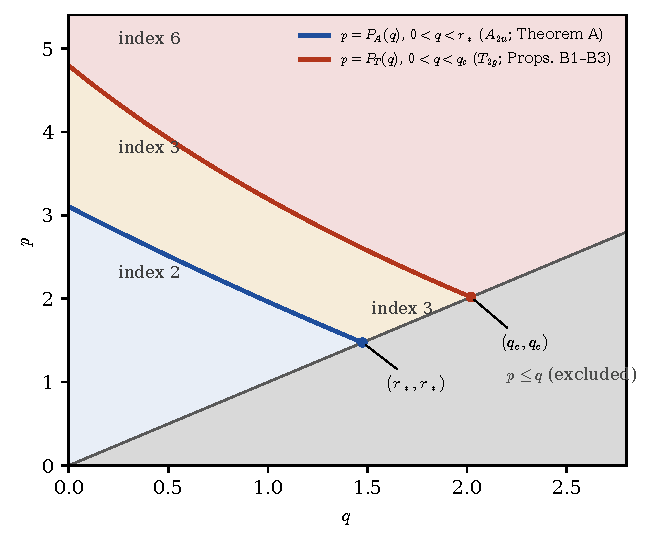
\includegraphics[width=0.62\textwidth]{figures/fig1_parameter_plane.pdf}
\caption{The parameter plane. The two transition curves of Paper~2, $p=P_A(q)$ for $0<q<\rstar$ and $p=P_T(q)$ for
$0<q<\qc$, end on the diagonal at $(\rstar,\rstar)$ and $(\qc,\qc)$ and never meet. The curves are drawn from their exact
definitions, evaluated at 30 significant digits by the project's root finders; their properties are proved in
Paper~2. The shading and the index labels illustrate Paper~2's index formula for the cube and are not a result of
this paper. The local branch results of this paper hold near each point of the two open curves.}
\label{fig:plane}
\end{figure}

\paragraph{Block signs on the $\Ttwog$ curve.} \Cref{tab:blocks} lists the signs that Paper~2's Theorem~2(b)--(d)
gives on $p=P_T(q)$, $0<q<\qc$. They are used only in \corBthree.

\begin{table}[h]
\centering\small
\caption{Hessian blocks of the cube on the physical $\Ttwog$ curve (frozen inputs from Paper~2).}\label{tab:blocks}
\begin{tabular}{lccl}
\toprule
block & dim & sign & source (Paper~2)\\
\midrule
$\Aonegg$ & 1 & $+$ & Lemma S\\
$\Eg$ & 2 & $+$ & Lemma S\\
$\Tonegg$ (rotations) & 3 & $0$, rigid, excluded & setup\\
$\Ttwog$ lower (critical) & 3 & $0$, the centre space $E_c$ & Lemmas T1, T3\\
$\Ttwog$ upper (noncritical copy) & 3 & $+$ & Lemma T1\\
$\Atwou$ & 1 & $-$ & Lemma T4\\
$\Eu$ & 2 & $-$ & Lemma E\\
$\Toneu$ (translations) & 3 & $0$, rigid, excluded & setup\\
$\Toneu$ (internal) & 3 & $+$ & Lemma S\\
$\Ttwou$ & 3 & $+$ & Lemma S\\
\bottomrule
\end{tabular}
\end{table}

\section{The $\Atwou$ pitchfork}\label{sec:a2u}

Fix $q\in(0,\rstar)$ and put $\mu=p-P_A(q)$. On the curve the slice kernel is $E_c=\Span\{\eA\}$: $\Atwou$ occurs once
in \eqref{eq:gamma24}, $\eA$ is an exact Hessian eigenvector with eigenvalue $V_{aa}=qW_q[h_A(p)-h_A(q)]$ for every
$p$, and no other block vanishes on $p=P_A(q)$ (Paper~2, Theorem~2).

\subsection{Symmetry of the $\Atwou$ direction}\label{sec:a2u-sym}

\begin{lemma}[exact symmetry facts]\label{lem:a0}
\begin{enumerate}[label=(\alph*)]
\item The stabiliser $\Sigma_A=\{R:D(R)\eA=\eA\}$ has $24$ elements ($E$, $8C_3$, $3C_2$, $6S_4$, $6\sigma_d$, no
inversion), i.e.\ $\Sigma_A\cong\Td$, and $\Fix(\Td)=\Span\{\ebr,\eA\}$.
\item Spatial inversion acts by $D(-I)\eA=-\eA$ and fixes $\ystar$.
\item $b:=D^3V[\eA,\eA,\cdot\,]=V_{aab}\,\ebr$ exactly, for every pair potential, and $\ebr$ is a Hessian eigenvector with
eigenvalue $V_{bb}=2qW_q(p-q)>0$.
\end{enumerate}
\end{lemma}
\begin{proof}
(a), (b) are computed from the $48$ matrices. (c): $\Atwou\otimes\Atwou=\Aonegg$, so $b$ is $\Oh$-invariant and lies in
the one-dimensional $\Fix(\Oh)=\Span\{\ebr\}$; the identity and the closed forms of $V_{aab}$, $V_{bb}$ are verified
component by component in $\R^{24}$ (\cref{app:closed}).
\end{proof}

By (b) and the equivariance of the reduction, $\Vred(a,\mu)=\Vred(-a,\mu)$ on $E_c$: the reduced potential is even
and every odd coefficient, in particular the cubic one, vanishes. By (c) the general Lyapunov--Schmidt formula for the
quartic coefficient,
\begin{equation}\label{eq:c4general}
\Vred(a,\mu)=\Vred(0,\mu)+\tfrac12\lambda(\mu)a^2+\tfrac{c_4(\mu)}{24}a^4+O(a^6),\qquad
c_4=D^4V[e,e,e,e]-3\langle b,H_\perp^{-1}b\rangle,
\end{equation}
collapses at $\mu=0$ to $c_4=V_{aaaa}-3V_{aab}^2/V_{bb}$.

\subsection{The quartic coefficient and Lemma M}

Each quantity in this formula is a difference $qW_q[g(p)-g(q)]$ of one-variable functions (\cref{app:closed}). A
second, scale-eliminated expression is more convenient for the sign. Put $x=2^{-r/2}$, $y=3^{-r/2}$, $S=3x+y+3$ and
\begin{equation}\label{eq:m}
m(r)=\frac{S\,(3r^3x+81r+(3r+2)y+126)-3r(3rx-y-9)^2}{16\,S^2}.
\end{equation}

\begin{lemma}[scale-eliminated form]\label{lem:foliation}
On the curve $p=P_A(q)$,
\begin{equation}\label{eq:c4m}
c_4(q)=\tfrac{16}{3}\,qW_q\,\bigl[m(P_A(q))-m(q)\bigr].
\end{equation}
\end{lemma}
\begin{proof}
Restrict to the $\Td$-symmetric shapes: two concentric regular tetrahedra of radii proportional to $e^{\mp u/2}$. The
logarithm $f(u)=p\log U_q-q\log U_p$ of the scale-free shape function $\Phi_{p,q}$ is even in $u$, and its fourth
Taylor coefficient is $f''''(0)=pq\,[m(q)-m(p)]$, with $m$ as in \eqref{eq:m} (the factor $r$ of the Taylor
coefficients of $U_r$ cancels exactly, so $m$ is analytic at $r=0$). A general exact lemma compares the quartic
coefficient of the full-energy reduction with that of the reduction along scaling orbits for an even function $F(a,b)$:
their difference is a multiple of $F_{aa}$ and therefore vanishes on the curve. Together with $V_*=-K\Phi_{p,q}^{1/(p-q)}$
(Paper~2, Proposition~2.1) and the reparametrisation between $u$ and $a$ this gives \eqref{eq:c4m}. The identity was
also confirmed exactly against $c_4=V_{aaaa}-3V_{aab}^2/V_{bb}$ by a zero polynomial remainder modulo the cleared curve
equation $h_A(p)=h_A(q)$, and numerically at $415$ curve points to relative $10^{-39}$.
\end{proof}

\begin{named}{Lemma M}[certified]\phantomsection\label{lem:M}
$m'(r)\ge L_{\min}=161457/262144=0.61590957\ldots>0$ for every $r\in[0,16/5]$.
\end{named}

The proof is an Arb ball-arithmetic certificate \citep{Johansson2017}: $64$ boxes with exact rational endpoints $k/20$,
a mean-value box test with an exactly derived $m''$, dyadic lower bounds, and an independent checker; it is described
in \cref{sec:cert} and \cref{app:certs}. Near $r=0$ the expansion $m'(0)=\frac{18}{49}+\frac{12}{49}\log2+\frac{57}{784}\log3>0$
and a separate certificate of $m''>0$ on $[0,1/8]$ give the bound independently of the main covering. A further
certified inequality, $h_A(16/5)<-6/7$ and $h_A'(16/5)<0$, combined with Paper~2's Lemma~A ($h_A(0^+)=-6/7$), gives
$0<q<\rstar<P_A(q)<16/5$ for all $0<q<\rstar$.

\begin{named}{Corollary M}\phantomsection\label{cor:M}
$c_4(q)>0$ for every $0<q<\rstar$; more precisely $c_4(q)\ge\frac{16}{3}L_{\min}\,qW_q\,(P_A(q)-q)>0$.
\end{named}
\begin{proof}
Both $q$ and $P_A(q)$ lie in $[0,16/5]$ and $P_A(q)>q$. By the mean value theorem and \lemM,
$m(P_A(q))-m(q)\ge L_{\min}(P_A(q)-q)$; insert into \eqref{eq:c4m}.
\end{proof}

\subsection{Theorem A}

\begin{named}{Theorem A}[the $\Atwou$ pitchfork]\phantomsection\label{thm:A}
Fix $q\in(0,\rstar)$. There are $\varepsilon>0$ and a neighbourhood $\mathcal N$ of $\ystar$ in $\mathcal S$ such that,
for $|\mu|<\varepsilon$, the equilibria of $V_p$ in $\mathcal N$ are exactly
\begin{enumerate}[label=(\arabic*)]
\item the cube $\ystar$, for every such $p$; and
\item for $\mu>0$ only, two further equilibria $x_\pm(p)=\ystar\pm a(p)\eA+w(p)$ with $a(p)>0$,
$w(p)=\beta(p)\ebr$, $\beta(p)=O(a(p)^2)$, and
\begin{equation}\label{eq:ampA}
a(p)^2=\frac{6\,qW_q\,|h_A'(P_A(q))|}{c_4(q)}\,\mu+O(\mu^2),\qquad c_4(q)>0\ \text{(\corM)}.
\end{equation}
\end{enumerate}
Each of $x_\pm$ consists of two concentric regular tetrahedra of unequal radii on inversion-related vertex-direction
sets and has point group $\Td$. Spatial inversion exchanges the complete branch configurations $x_+$ and $x_-$; it does
not exchange the unequal-radius shells within one fixed configuration. The bifurcation is a $\Z_2$-symmetric
pitchfork, supercritical in the reduced-energy convention: for $0<\mu<\varepsilon$, $\Vred(\cdot,\mu)$ has a strict
local maximum at $a=0$ and strict local minima at $a=\pm a(p)$.
\end{named}

\begin{proof}
By \cref{sec:model} the equilibria near $\ystar$ in $\mathcal S$ are the critical points of the one-dimensional
reduced potential on $E_c=\Span\{\eA\}$, which is analytic and even (\cref{lem:a0}(b)). Hence
$\partial_a\Vred=a\,G(a^2,\mu)$ with $G$ analytic and $G(z,\mu)=\lambda(\mu)+\frac{c_4(\mu)}{6}z+O(z^2)$. Because $\eA$
is an exact Hessian eigenvector for every $p$, $\lambda(\mu)=qW_q[h_A(P_A(q)+\mu)-h_A(q)]$ exactly, so $\lambda(0)=0$
and $\lambda'(0)=qW_q\,h_A'(P_A(q))<0$ (Paper~2, Lemma~A: $h_A$ decreases strictly on $(\rstar,\infty)$). Thus
$G(0,0)=0$, $G_\mu(0,0)=\lambda'(0)\ne0$ and $G_z(0,0)=c_4/6>0$. By the implicit function theorem the zeros of $G$ near
$(0,0)$ form one analytic curve $\mu=\mu_*(z)$ with $\mu_*'(0)=-G_z/G_\mu=-c_4/(6\lambda'(0))>0$. Hence $a^2=z>0$ forces
$\mu>0$, and for each small $\mu>0$ there is exactly one $z=a(p)^2$, given by \eqref{eq:ampA}; for $\mu\le0$ there is
none. Next, $\partial_a^2\Vred=G+2a^2G_z$: at $a=0$ it equals $\lambda(\mu)<0$ for $\mu>0$, and on the branch, where
$G=0$, it equals $\frac{c_4}{3}a(p)^2+O(\mu^2)=-2\lambda(\mu)+O(\mu^2)>0$.

Equivariance of the reduction gives $D(R)x(a)=x(\sigma(R)a)$, so the solution $w$ lies in $\Fix(\Td)\cap\eA^\perp=
\Span\{\ebr\}$, $D(-I)$ maps $x_+$ to $x_-$, and each $x_\pm$ is fixed exactly by $\Td$ within $\Oh$. Concretely, $x_\pm$
consists of the even and the odd tetrahedron of the cube scaled about the centre by
$\frac12+(\beta\pm a)/\sqrt{24}$ and $\frac12+(\beta\mp a)/\sqrt{24}$. Since $a\ne0$ the radii differ, so no symmetry of
a fixed configuration exchanges the two shells, and the point group is the symmetry group $\Td$ of a regular tetrahedron,
in agreement with the computed stabiliser. Spatial inversion preserves radii; it maps the vertex directions of one
tetrahedron to those of the other, and it maps $x_+$ to $x_-$, not one shell of $x_+$ onto the other. The conditions
$G_\mu\ne0$, $G_z\ne0$ are the recognition conditions of the $\Z_2$-symmetric pitchfork \citep{GolubitskySchaeffer1985};
the argument uses only the implicit function theorem.
\end{proof}

\begin{remark}[conventions]\label{rem:supercritical}
``Supercritical'' refers to the reduced-energy convention: the gradient flow $\dot a=-\partial_a\Vred=\nu a-\frac{c_4}{6}a^3+\dots$,
$\nu=-\lambda(\mu)$, has the normal form $\dot x=\nu x-x^3$ when $c_4>0$, and the branch exists on the side where the
cube has lost minimality along $\eA$; the branch points are minima of the one-dimensional reduced potential. The cube
is already a saddle of $V_p$ in $\mathcal T^\perp$ (index at least $2$), so \thmA\ is not a stability statement in
the full configuration space and claims no Morse index of $x_\pm$.
\end{remark}

\section{The critical $\Ttwog$ representation and its invariants}\label{sec:t2g}

Fix $q\in(0,\qc)$ and put $\mu=p-P_T(q)$. On the curve $K$ is singular with $\tr K>0$, so its kernel is spanned by a
unit vector $n=(n_u,n_v)$, which we fix at $\mu=0$ in the gauge $n_u>0$ (justified in \cref{sec:d3d}). The critical
vectors and their partners are
\begin{equation}\label{eq:ek}
e_k=n_u\,\uh_k+n_v\,\vh_k,\qquad f_k=-n_v\,\uh_k+n_u\,\vh_k\qquad(k=1,2,3),
\end{equation}
and $E_c=\Span\{e_1,e_2,e_3\}$ is the slice kernel at $\mu=0$ (Paper~2, Theorem~2: no other block vanishes on the
curve). Numerically $n\approx(0.9997,\,0.02\text{--}0.03)$ along the curve: the critical mode is almost a pure shear with
a small opposite translation of the two tetrahedra. We write $a=(a_1,a_2,a_3)$ for the coordinates of
$\sum_ka_ke_k\in E_c$; by \eqref{eq:TR}, $\Oh$ acts on $a$ by $T(R)=\sigma(R)R$.

\subsection{Invariant theory}

\begin{lemma}[invariants and isotropy]\label{lem:invariants}
Let $G_T=\{T(R):R\in\Oh\}$ ($24$ matrices).
\begin{enumerate}[label=(\alph*)]
\item The $G_T$-invariant polynomials of degree $1,\dots,6$ have dimensions $0,1,1,2,1,3$. Degree $2$ is spanned by
$I_2=|a|^2$, degree $3$ by $I_3=a_1a_2a_3$, and degree $4$ by $I_2^2$ and $I_4=a_1^4+a_2^4+a_3^4$.
\item The isotropy subgroups of $\Oh$ on $E_c$, their fixed spaces and representatives are as in \cref{tab:isotropy}. The
stabiliser in $\Oh$ of $\sum_ka_ke_k\in\R^{24}$ equals the stabiliser of $a$ under $T$.
\end{enumerate}
\end{lemma}
\begin{proof}
(a) Reynolds averaging over $G_T$ applied to all monomials of each degree \citep{Sturmfels2008}, in exact arithmetic.
(b) Stabilisers of all integer vectors in $[-2,2]^3$ computed from the matrices; element types classified from
the matrices; the $24$-dimensional stabilisers checked at representatives with symbolic $n$.
\end{proof}

\begin{table}[h]
\centering\small
\caption{Isotropy on the critical $\Ttwog$ space (computed). Only the two axial types give branches by the
equivariant branching lemma.}\label{tab:isotropy}
\begin{tabularx}{\textwidth}{>{\raggedright\arraybackslash}p{3.3cm}cccc>{\raggedright\arraybackslash}X}
\toprule
isotropy & order & conjugates & $\dim\Fix$ & representative $a$ & action of the normaliser on the axis\\
\midrule
$\Dthreed$ & 12 & 4 & 1 & $(1,1,1)$ & trivial; $I_3\ne0$ on the axis\\
$\Dtwoh$ (one $C_4$ axis, two face diagonals) & 8 & 3 & 1 & $(1,0,0)$ & normaliser $\Dfourh$ contains $a\mapsto-a$\\
$C_{2h}$ (face-diagonal axis) & 4 & 6 & 2 & $(1,1,0)$ & not axial\\
$C_i$ & 2 & 1 & 3 & generic & ---\\
\bottomrule
\end{tabularx}
\end{table}

On the $\Dtwoh$ axis some element of the normaliser reverses $a$, so the reduced equation there is odd (pitchfork
type); on the $\Dthreed$ axis no element reverses $a$, and $I_3$ does not vanish there. Because $I_3$ is invariant,
$\nabla I_3$ is a nonzero quadratic equivariant; this is the setting of Ihrig and Golubitsky \citep{IhrigGolubitsky1984}.
Their theorem concerns stability (generic instability of axial branches near the bifurcation); it does not decide
whether a branch is transcritical, and it is not used in any proof below.

\subsection{The reduced potential on $E_c$}

With the Lyapunov--Schmidt reduction of \cref{sec:model} on the slice (here $H_{WW}$ is invertible but indefinite, with
index $3$; \cref{tab:blocks}) and the invariance of $\Vred$ under $G_T$, \cref{lem:invariants}(a) gives the normal form
\begin{equation}\label{eq:normalform}
\Vred(a,\mu)=V_0(\mu)+\tfrac12\lambda(\mu)I_2+\kappa(\mu)I_3+\alpha(\mu)I_2^2+\beta(\mu)I_4+O(|a|^5),
\end{equation}
with coefficients analytic in $\mu$. Since $w=O(|a|^2)$, the cubic part is $\frac16D^3V[x,x,x]$ with $x=\sum a_ke_k$, so
$\kappa(0)=\kappa:=D^3V[e_1,e_2,e_3]$ (\cref{sec:d3d}). The quartic coefficients $\alpha,\beta$ are determined in
\cref{sec:index}; their sum is $c_4/24$, where $c_4$ is the quartic coefficient on the $\Dtwoh$ axis (\cref{sec:d2h}).

\subsection{Transversality}

Let $\tau:=n^{\mathsf T}\partial_pK\,n=qW_q\,n^{\mathsf T}M'(P_T(q))\,n$ at $\mu=0$.

\begin{lemma}[transversality]\label{lem:tau}
$\tau<0$ for every $0<q<\qc$, and $\lambda(0)=0$, $\lambda'(0)=\tau$ in \eqref{eq:normalform}.
\end{lemma}
\begin{proof}
On the curve $N=M(p)-M(q)$ is symmetric and singular with kernel $n$, so $\adj N=\tr(N)\,nn^{\mathsf T}$ (exact
identity) and $\partial_pD=\tr(N)\,n^{\mathsf T}M'(p)\,n$. By Lemma~T1, $\tr N>0$; by Lemma~T3, $\partial_pD(P_T(q),q)<0$.
Hence $n^{\mathsf T}M'(p)n<0$ and $\tau<0$. For the second statement: $\lambda(\mu)$ is the Schur complement
$\det K(p)/(f^{\mathsf T}K(p)f)$ with $f=(-n_v,n_u)$ (the breathing and other blocks do not couple at second order), so
$\lambda(0)=0$ and $\lambda'(0)=n^{\mathsf T}\partial_pK\,n=\tau$; this is checked symbolically for a generic $K(\mu)$.
\end{proof}

\section{The cubic coefficient and the $\Dthreed$ transcritical branches}\label{sec:d3d}

\subsection{Exact trilinear structure}

Write $\phi(r)=\psi(r^2)$ and evaluate $\psi^{(k)}$ at $\sigma=|r|^2\in\{1,2,3\}$. Of the $216$ values
$D^3V[b_i,b_j,b_k]$ on the six basis vectors \eqref{eq:t2gbasis}, computed for a generic $\psi$ before any symmetry is
used, exactly $48$ are nonzero, all with $\{i,j,k\}=\{1,2,3\}$, and they reduce to four coefficients:
\begin{equation}\label{eq:tcoeffs}
\begin{aligned}
t_{uuu}&=-12\psi''(2)-12\psi''(3)-32\psi'''(3), & t_{uuv}&=-\sqrt2\bigl(10\psi''(3)+16\psi'''(3)\bigr),\\
t_{uvv}&=-8\psi''(1)-8\psi''(3)-16\psi'''(3), & t_{vvv}&=-8\sqrt2\,\psi'''(3),
\end{aligned}
\end{equation}
\begin{equation}\label{eq:kappa}
\kappa=t_{uuu}n_u^3+3t_{uuv}n_u^2n_v+3t_{uvv}n_un_v^2+t_{vvv}n_v^3 .
\end{equation}
An independent computation of the full third-derivative tensor in the $24$ raw coordinates reproduces these
coefficients and gives, for symbolic $n$ and $\psi$, $D^3V[x,x,x]=6\kappa\,a_1a_2a_3$ for $x=\sum a_ke_k$: the cubic
restriction to $E_c$ is exactly a multiple of $I_3$.

\subsection{Factorisation and Lemma K}

At the unit-edge equilibrium each coefficient is a difference form $t_m=qW_q[g_m(p)-g_m(q)]$ (\cref{app:closed}). Let
$\hat f(p,q)=(f(p)-f(q))/(p-q)$ with $\hat f(q,q)=f'(q)$, an analytic function of $(p,q)$. Then
$K=qW_q(p-q)\Mhat$ with $\Mhat=\hat M(p,q)$, the curve is $\Dt(q,\delta):=\det\Mhat(q+\delta,q)=0$ with $\delta=p-q>0$,
and its closure adds the corner $(\qc,\qc)$, where $\Dt=\det M'(\qc)=0$ (Lemma~T2). The cubic coefficient factorises:
\begin{equation}\label{eq:kappafact}
\kappa=qW_q\,(p-q)\,\khat,\qquad \khat=\frac{\hat g_{uuu}+3\rho\,\hat g_{uuv}+3\rho^2\hat g_{uvv}+\rho^3\hat g_{vvv}}{(1+\rho^2)^{3/2}},\qquad
\rho=-\frac{\Mhat_{12}}{\Mhat_{22}},
\end{equation}
for the unit kernel vector $n=(1,\rho)/\sqrt{1+\rho^2}$; indeed $\Mhat(1,\rho)^{\mathsf T}=(\det\Mhat/\Mhat_{22},0)^{\mathsf T}$
exactly, so $(1,\rho)$ spans the kernel wherever $\Mhat_{22}\ne0$. The raw $\kappa$ vanishes at both ends of the curve
through the factors $q$ and $p-q$; the carrier $\khat$ is analytic on the closed curve. The sign of $\kappa$ changes
under $n\mapsto-n$; only $\kappa\ne0$ is gauge invariant.

\begin{named}{Lemma K}[certified]\phantomsection\label{lem:K}
On the closed physical $\Ttwog$ curve, i.e.\ $p=P_T(q)$ for $0\le q<\qc$ together with the corner $p=q=\qc$,
\[
\khat\ge 1311719/536870912=0.0024432670\ldots>0\qquad\text{and}\qquad \Mhat_{22}>0 .
\]
Hence $n_u\ne0$ on the whole curve, one chart covers it, and $\kappa(q)\ne0$ for every $0<q<\qc$; in the gauge
$n_u>0$, $\kappa(q)>0$.
\end{named}

The certificate (\cref{sec:cert}, \cref{app:certs}) covers $q\in[0,101/50]$ by $222$ boxes with exact rational
endpoints. On each box a parametric interval Newton step proves that $\Dt(q,\cdot)$ has exactly one zero in a recorded
$\delta$-ball for every $q$ in the box, and the carrier is enclosed above a dyadic lower bound. The endpoint values are
$\khat(0)=0.00287951258\ldots$ and $\khat(\qc)=0.00689178231\ldots$. Every box except the corner box has a positive
$\delta$-ball, so its zero is $P_T(q)$ by Lemma~T3; on the corner box continuity and $\Dt(q,0)=\det M'(q)>0$ for $q<\qc$
(Lemma~T2) identify the zero with $P_T(q)-q$ for $q<\qc$ and with the corner at $q=\qc$.

\subsection{Proposition B1}

\begin{named}{Proposition B1}[the $\Dthreed$ branches]\phantomsection\label{prop:B1}
Fix $q\in(0,\qc)$, the gauge $n_u>0$, and $\kappa,\tau$ at $\mu=0$; then $\kappa>0$ (\lemK) and $\tau<0$
(\cref{lem:tau}). In $\ystar+\Fix(\Dthreed)$ near $\ystar$, for small $|\mu|$, the equilibria of $V_p$ are exactly the cube
and one branch
\[
x(\mu)=\ystar+s_*(\mu)(e_1+e_2+e_3)+w(\mu),\qquad s_*(\mu)=-\frac{\tau}{\kappa}\,\mu+O(\mu^2),
\]
with $w(\mu)\in\Span\{\ebr,f_1+f_2+f_3\}$. The branch exists for both signs of $\mu$ and $s_*(\mu)\ne0$ for $\mu\ne0$; it
crosses the cube transversally, so the bifurcation is \emph{transcritical}. In this gauge $s_*>0$ for $p>P_T(q)$ and
$s_*<0$ for $p<P_T(q)$. The same holds on each of the four $\Dthreed$ axes, which are conjugate under $\Oh$.
\end{named}

\begin{proof}
$\Fix(\Dthreed)=\Span\{\ebr,\sum_k\uh_k,\sum_k\vh_k\}$ is three-dimensional and contains no rigid motion; by symmetric
criticality its equilibria are those of $V$ restricted to it. At $\mu=0$ the Hessian there has kernel
$\Span\{e_1+e_2+e_3\}$ ($\Fix(\Dthreed)$ meets $E_c$ only on the diagonal, and the other blocks are nonzero). The
one-dimensional reduction gives, since $|a|^2=3s^2$ and $a_1a_2a_3=s^3$ on the axis,
\[
v(s,\mu)=v(0,\mu)+\tfrac32\lambda(\mu)s^2+\kappa(\mu)s^3+O(s^4),\qquad \partial_sv=3s\,G(s,\mu),\quad G=\lambda(\mu)+\kappa(\mu)s+O(s^2),
\]
with $\lambda(0)=0$, $\lambda'(0)=\tau$ (\cref{lem:tau}). $G(0,0)=0$, $G_s(0,0)=\kappa\ne0$ and $G_\mu(0,0)=\tau\ne0$; by the
implicit function theorem the nontrivial zeros near $(0,0)$ form one curve $s=s_*(\mu)$ with $s_*'(0)=-\tau/\kappa\ne0$.
The trivial solution $s=0$ is the cube.
\end{proof}

Both coefficients are needed: $\kappa\ne0$ for the implicit function theorem, and $\tau\ne0$ so that the branch leaves
the cube on both sides. To first order the displacement $s(e_1+e_2+e_3)$ moves vertex $s$ by
$-\frac{sn_u}{4}(J-I)s-\frac{sn_v\sqrt2}{4}(s_1s_2s_3)(1,1,1)$, $J$ the all-ones matrix: the cube is scaled by $1-sn_u$
along the body diagonal $(1,1,1)$ and by $1+sn_u/2$ across it, and the two tetrahedra shift oppositely along that
diagonal with the small weight $n_v$. For $p>P_T(q)$ the cube is compressed along one body diagonal, for $p<P_T(q)$
elongated (\cref{fig:modes}). No stability statement is made in \propBone; the Morse index of these branches is not
determined in this paper (a consistency check appears in \cref{rem:d3d}).

\section{The $\Dtwoh$ pitchfork branches}\label{sec:d2h}

Keep $q\in(0,\qc)$, $\mu=p-P_T(q)$ and the gauge $n_u>0$. The $\Dtwoh$ axis of $E_c$ is $a=(s,0,0)$, i.e.\ the
displacement $s\,e_1$.

\subsection{The fixed space}

\begin{lemma}[exact symmetry audit of the $\Dtwoh$ axis]\label{lem:fix}
Let $\Sigma=\{R\in\Oh:D(R)e_1=e_1\}$.
\begin{enumerate}[label=(\alph*)]
\item $\Sigma$ has order $8$ (elements $E$, $C_4^2$, $i$, $\sigma_h$, $2C_2'$, $2\sigma_d$): it is the $\Dtwoh$ with
$C_2$ axes $x$, $(0,1,1)$, $(0,1,-1)$, for every $n$.
\item $\Fix_{\R^{24}}(\Sigma)=\Span\{\Ahat,\Ehat,e_1,f_1\}$ (orthonormal), where $\Ahat=E_{\mathrm{br}}/\sqrt{24}$
($\Aonegg$), $\Ehat(s)=(2s_1,-s_2,-s_3)/\sqrt{48}$ (the tetragonal $\Eg$ strain along the axis), and $e_1,f_1$ are one
direction from each $\Ttwog$ copy. Isotypically,
\[
\Fix(\Sigma)=\Aonegg\oplus\Eg\oplus\Ttwog^{(1)}\oplus\Ttwog^{(2)}\quad(\text{one fixed direction each}),
\]
and no rigid motion is fixed.
\item $b:=D^3V[e_1,e_1,\cdot\,]\in\Aonegg\oplus\Eg$: $b=b_A\Ahat+b_E\Ehat$ exactly, with $\langle b,e_1\rangle=\langle b,f_1\rangle=0$.
\item The $8$ elements of $\Oh$ that map $e_1$ to $-e_1$ form, with $\Sigma$, the normaliser $N(\Sigma)\cong\Dfourh$; each
acts on $(\Ahat,\Ehat,e_1,f_1)$ as $\operatorname{diag}(1,1,-1,-1)$.
\item In the basis $(\Ahat,\Ehat,\uh_1,\vh_1)$ the Hessian restricted to $\Fix(\Sigma)$ is $\operatorname{diag}(h_A,h_E)\oplus K$,
where $h_A$, $h_E$ are the $\Aonegg$ and $\Eg$ eigenvalues of the cube.
\end{enumerate}
\end{lemma}
\begin{proof}
All items are computed exactly from the $\Oh$ action on $\R^{24}$, with $n_u,n_v$ symbolic and a generic pair
potential: the stabiliser from the $48$ matrices, the fixed space from the projector $\frac18\sum_{g\in\Sigma}D(g)$ (rank
$4$) and the ranks of its products with the isotypic projectors, and $b$ as a $24$-vector of linear forms in
$\psi^{(k)}(\sigma)$. For (c) there is also a structural reason: $b$ is the image of $e_1\otimes e_1$ under an
$\Oh$-equivariant map, $\operatorname{Sym}^2(\Ttwog)=(\Aonegg\oplus\Eg)\oplus\Ttwog$, and the $\Ttwog$ component of
$\operatorname{Sym}^2$ is $(a_2a_3,a_3a_1,a_1a_2)$, which vanishes at $(1,0,0)$ (on the $\Dthreed$ axis it does not; this
is the $I_3$ structure seen from the other side).
\end{proof}

\begin{remark}\label{rem:fixspace}
The fixed space contains the noncritical same-axis $\Ttwog$ direction $f_1$ and exactly one $\Eg$ direction (the
strain $\operatorname{diag}(0,1,-1)$ is not $\Sigma$-fixed). An informal description used in early planning,
$\Span\{e_{\mathrm{crit}},\Aonegg,\Eg^{(1)},\Eg^{(2)}\}$, omitted $f_1$ and included a second $\Eg$ direction; only the
dimension agrees. The comparison is recorded in the development documentation of the release package.
\end{remark}

\subsection{The quartic coefficient and Lemma Q}

By \cref{lem:fix}(d) the reduced potential on the axis is even, and $D^3V[e_1,e_1,e_1]=0$. Eliminating
$w\in\Span\{\Ahat,\Ehat,f_1\}$ at second order, with $b\in\Span\{\Ahat,\Ehat\}$ and $\Ahat,\Ehat$ eigenvectors of the full
Hessian, gives
\begin{equation}\label{eq:c4D2h}
c_4=D^4V[e_1^4]-3\langle b,H_\perp^{-1}b\rangle=D^4V[e_1^4]-3\frac{b_A^2}{h_A}-3\frac{b_E^2}{h_E}.
\end{equation}
The denominators are positive for all $p>q>0$ (Paper~2, Lemma~S). The value of \eqref{eq:c4D2h} was confirmed by three
independent routes: the symmetry-adapted formula, a raw $24$-dimensional computation with no symmetry (exact in
SymPy \citep{SymPy2017} for symbolic $n$, and numerically with a spectral pseudo-inverse), and a derivative-free
nonlinear reduction in the four $\Sigma$-orbit coordinates; at five curve points they agree to relative $10^{-36}$ or
better. All terms are difference forms (\cref{app:closed}), each carries the factor $qW_q(p-q)$, and
\begin{equation}\label{eq:c4fact}
c_4=qW_q\,(p-q)\,\cfhat,\qquad
\cfhat=\frac{\widehat Q(1,\rho)-\frac32\,\widehat b_A(1,\rho)^2-3\,\widehat b_E(1,\rho)^2/\widehat h_E}{(1+\rho^2)^2},
\end{equation}
with the divided differences $\hat f$ of \cref{sec:d3d}, the chart $\rho=-\Mhat_{12}/\Mhat_{22}$, $\widehat h_A=2$ exactly, and
$\widehat Q(n)=\sum_j\binom4j n_u^{4-j}n_v^j\widehat Q_j$. Unlike $\kappa$, $c_4$ does not depend on the gauge.

\begin{named}{Lemma Q}[certified]\phantomsection\label{lem:Q}
On the whole closed physical $\Ttwog$ curve ($p=P_T(q)$, $0\le q<\qc$, and the corner $p=q=\qc$), $\cfhat>0$, together with
$\widehat h_E>0$ and $\Mhat_{22}>0$. More precisely $\cfhat\ge955723/262144=3.6457\ldots$ on every curve box,
$\cfhat(0)=3.7993380378\ldots$ and $\cfhat(\qc)=4.3770354906\ldots$. At $q=0$ the divided differences are
$(f(P_T(0))-f(0))/P_T(0)$; at the corner they are the derivatives $f'(\qc)$.
\end{named}

The certificate uses the $222$ curve boxes and $\delta$-balls of the \lemK\ certificate unchanged (hash-pinned), re-verifies
each ball by a strict interval Newton inclusion, encloses the divided differences without dividing by $\delta$, and
certifies both endpoints directly; an independent checker re-derives all functions and uses no Taylor series
(\cref{sec:cert}).

\begin{corollary}[sign of $c_4$]\label{cor:c4}
$c_4(q)=qW_q\,(P_T(q)-q)\,\cfhat(q)>0$ for every $0<q<\qc$, since $q>0$, $W_q>1$ and $P_T(q)>q$ (Lemma~T3). The raw $c_4$
vanishes at both ends through the factors $q$ and $p-q$; no sign of the raw $c_4$ is claimed there.
\end{corollary}

\subsection{Proposition B2}

\begin{named}{Proposition B2}[the $\Dtwoh$ pitchfork]\phantomsection\label{prop:B2}
Fix $q\in(0,\qc)$. Then $\tau<0$ and $c_4>0$. There are $\varepsilon>0$ and $\mu_0>0$ such that for $|\mu|<\mu_0$ the
equilibria of $V_p$ in $\ystar+\Fix(\Sigma)$ within distance $\varepsilon$ of $\ystar$ are exactly
\begin{itemize}
\item the cube, for every $\mu$;
\item for $\mu>0$ only, two further equilibria $x_\pm(\mu)=\ystar\pm s_*(\mu)e_1+w(\pm s_*(\mu),\mu)$ with $s_*(\mu)>0$ and
\begin{equation}\label{eq:ampD2h}
s_*(\mu)^2=-\frac{6\tau}{c_4}\,\mu+O(\mu^2);
\end{equation}
\item for $\mu\le0$, no other equilibrium.
\end{itemize}
$x_+$ and $x_-$ are exchanged by each element of $N(\Sigma)\setminus\Sigma$, and each has isotropy exactly $\Sigma\cong\Dtwoh$ in
$\Oh$. The branch is a $\Z_2$-symmetric pitchfork, supercritical in the reduced-energy axial convention, opening towards
$p>P_T(q)$. Along the axial reduced coordinate, $\partial_s^2\Vred=\tau\mu+O(\mu^2)<0$ at the cube for $\mu>0$ and
$\partial_s^2\Vred=-2\tau\mu+O(\mu^2)>0$ at $x_\pm(\mu)$. The same holds on each of the three $\Dtwoh$ axes.
\end{named}

\begin{proof}
\emph{Reduced equation.} Use orthonormal coordinates $(s,w_A,w_E,w_f)$ along $(e_1,\Ahat,\Ehat,f_1)$ on $\ystar+\Fix(\Sigma)$.
By symmetric criticality the $\Sigma$-symmetric equilibria are the critical points of $V$ restricted to this affine space.
By \cref{lem:fix}(e) the $s$-row of the Hessian is $(k_{ss},0,0,k_{sf})$ with $(k_{ss},k_{sf},k_{ff})=(n^{\mathsf T}Kn,n^{\mathsf T}Kf,f^{\mathsf T}Kf)$; at
$\mu=0$, $k_{ss}=k_{sf}=0$ and the other eigenvalues $h_A$, $h_E$, $k_{ff}=\tr K$ are positive (Lemmas~S, T1). The
Lyapunov--Schmidt solution $w(s,\mu)$ is unique and analytic, with $w(0,\mu)=0$, and $\Vred(s,\mu)=V(\ystar+se_1+w(s,\mu))$.
Each $g\in N(\Sigma)\setminus\Sigma$ maps $(s,w_A,w_E,w_f)$ to $(-s,w_A,w_E,-w_f)$ and preserves $V$, so by uniqueness
$\Vred(-s,\mu)=\Vred(s,\mu)$ and
\begin{equation}\label{eq:VredD2h}
\Vred(s,\mu)=V_0(\mu)+\tfrac12\lambda(\mu)s^2+\tfrac{c_4}{24}s^4+O(s^6,\mu s^4,\mu^2s^2),\qquad
\partial_s\Vred=s\,G(s^2,\mu),
\end{equation}
\[
G(z,\mu)=\lambda(\mu)+\tfrac{c_4}{6}\,z+O(z^2,\mu z,\mu^2),
\]
where $\lambda(\mu)=k_{ss}-k_{sf}^2/k_{ff}=\det K(p)/(f^{\mathsf T}K(p)f)$, so $\lambda(0)=0$ and $\lambda'(0)=\tau<0$
(\cref{lem:tau}), and the quartic coefficient at $\mu=0$ is \eqref{eq:c4D2h}, positive by \cref{cor:c4}.

\emph{Branch side.} $G(0,0)=0$, $G_\mu(0,0)=\tau\ne0$, $G_z(0,0)=c_4/6>0$. By the analytic implicit function theorem the
zeros of $G$ near $(0,0)$ form one curve $\mu=\mu_*(z)$ with $\mu_*'(0)=-c_4/(6\tau)>0$; inverting,
$z=-(6\tau/c_4)\mu+O(\mu^2)$. For small $s\ne0$, $x=\ystar+se_1+w(s,\mu)$ is an equilibrium if and only if $\mu=\mu_*(s^2)>0$,
so no nontrivial equilibrium exists for $\mu\le0$, and for small $\mu>0$ there is exactly one $z>0$ and exactly two
solutions $s=\pm s_*(\mu)$, $s_*=\sqrt z$. The side $\mu>0$ follows from the signs of $\tau$ and $c_4$; flipping either
sign would flip it.

\emph{Pitchfork and convention.} The cube exists for both signs of $\mu$, the pair $\pm s_*$ only for $\mu>0$, and every
$g\in N(\Sigma)\setminus\Sigma$ maps $x_+$ to $x_-$; $N(\Sigma)/\Sigma\cong\Z_2$ acts on the axis by $s\mapsto-s$. In the
reduced-energy axial convention of \cref{rem:supercritical} (with $\nu=-\lambda(\mu)$) the pitchfork is supercritical
because $c_4>0$: the pair exists where the cube's axial reduced curvature is negative, and consists of minima of
$\Vred(\cdot,\mu)$. The type is the sign of $c_4$ and does not depend on the orientation of $p$.

\emph{Axial curvature.} $\partial_s^2\Vred=G(s^2,\mu)+2s^2G_z(s^2,\mu)$. At the cube this is $\lambda(\mu)=\tau\mu+O(\mu^2)$;
at $s=\pm s_*$, where $G=0$, it is $2z(c_4/6+O(z,\mu))=-2\tau\mu+O(\mu^2)$.

\emph{Isotropy.} For every $R\in\Oh$ the rank of $(D(R)-I)[\uh_1,\vh_1]$ is $0$ if $R\in\Sigma$ and $2$ otherwise, and the $\Ttwog$
projector commutes with $D(R)$, kills $\Ahat,\Ehat$ and fixes $\uh_1,\vh_1$. Every point of $\ystar+\Fix(\Sigma)$ with a nonzero
$(\uh_1,\vh_1)$-component therefore has isotropy exactly $\Sigma$; on the branch that component is
$\pm s_*e_1+O(s_*^3)f_1\ne0$.
\end{proof}

\paragraph{Geometry.} The following is what is rigorously supported near the cube.
\begin{itemize}
\item \emph{Point group.} $x_\pm$ have point group exactly $\Dtwoh$ (not $\Dfourh$, not $\Oh$), and the branch stays
$\Dtwoh$-symmetric for all small $\mu>0$.
\item \emph{Not a cuboid.} $\Sigma$ contains only four of the eight diagonal sign matrices, and
$\Fix(\Sigma)\cap\Fix(\Z_2^3)=\Span\{\Ahat,\Ehat\}$, where $\Fix(\Z_2^3)=\Aonegg\oplus\Eg$ is the cuboid family of Paper~2. Since the
$e_1$-component of $x_\pm$ is nonzero, the branch configurations are not cuboids.
\item \emph{First order.} $\pm s_*e_1$ moves vertex $s$ by $\mp\frac{s_*n_u}{4}(0,s_3,s_2)\mp\frac{s_*n_v\sqrt2}{4}(s_1s_2s_3)(1,0,0)$.
The first term maps each cross-section $x=\text{const}$ by $(y,z)\mapsto(y-\varepsilon z,z-\varepsilon y)$,
$\varepsilon=\pm s_*n_u/2$: the square becomes a rhombus (four equal sides, diagonals scaled by $1-\varepsilon$ along
$(0,1,1)$ and $1+\varepsilon$ along $(0,1,-1)$), i.e.\ the cross-sections are sheared, and $x_+$, $x_-$ are the two rhombi
with the diagonals exchanged. The second term translates the two tetrahedra in opposite directions along $x$ with
weight $n_v$, the opposite-translation component of the critical mode ($n_v\approx0.020$--$0.028$ numerically; that
$n_v\ne0$ on the whole curve is not certified).
\item \emph{Second order.}
\[
x_\pm(\mu)-\ystar=\pm s_*e_1+s_*^2(\omega_A\Ahat+\omega_E\Ehat)+O(s_*^3),\qquad
(\omega_A,\omega_E)=-\tfrac12(b_A/h_A,\,b_E/h_E):
\] the second-order corrections lie in $\Aonegg\oplus\Eg$ (a breathing and a
tetragonal strain along $x$), and the $f_1$-component is $O(s_*^3)$.
\end{itemize}

\begin{figure}[t]
\centering
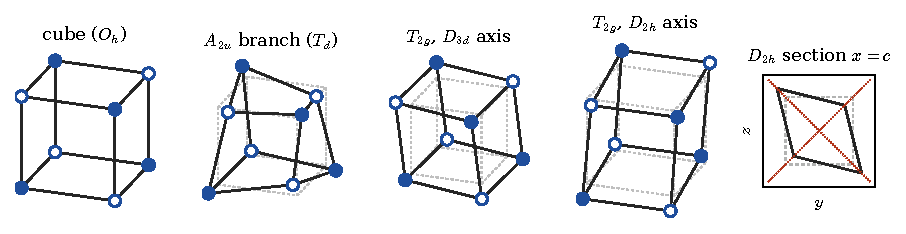
\includegraphics[width=\textwidth]{figures/fig2_modes.pdf}
\caption{First-order shapes of the branch configurations (amplitudes exaggerated; dashed: the cube). Filled and open
circles mark the even and odd tetrahedra. From left: the cube; the $\Atwou$ branch of \thmA, two concentric regular
tetrahedra of unequal radii on inversion-related vertex-direction sets ($\Td$); the $\Dthreed$ branch of \propBone\
(compressed along a body diagonal for $p>P_T(q)$); the $\Dtwoh$ branch of \propBtwo; and a cross-section $x=c$ of the
$\Dtwoh$ branch, in which the square becomes a rhombus (not a rectangle; the configuration is not a cuboid). The
displacements are computed from the exact first-order fields with the kernel vector $n$ at $q=0.8$; the opposite
translation of the tetrahedra (weight $n_v\approx0.025$) is too small to be visible at this scale.}
\label{fig:modes}
\end{figure}

\begin{figure}[t]
\centering
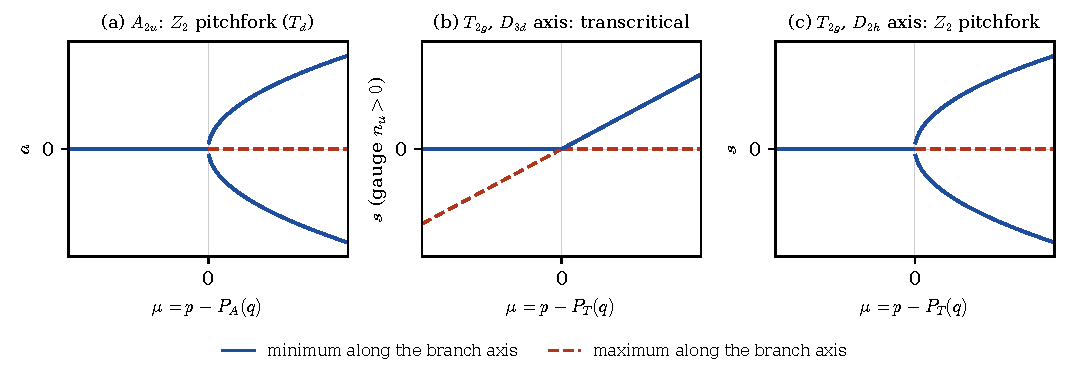
\includegraphics[width=\textwidth]{figures/fig3_bifurcation_diagrams.pdf}
\caption{Local bifurcation diagrams (leading-order normal forms; axes in arbitrary units). (a) $\Atwou$: $a^2\propto\mu$
for $\mu=p-P_A(q)>0$ (\thmA). (b) $\Dthreed$ axis: $s_*=-(\tau/\kappa)\mu$, plotted in the gauge $n_u>0$ where $\kappa>0$,
$\tau<0$ (\propBone). (c) $\Dtwoh$ axis: $s_*^2=-(6\tau/c_4)\mu$ for $\mu=p-P_T(q)>0$ (\propBtwo). Solid and dashed lines mark
minima and maxima of the one-dimensional reduced potential along the branch axis (the reduced-energy axial
convention). This is not stability in $\R^{24}$: the cube is a saddle throughout, and the $\Dtwoh$ branch points have
Morse index $4$ (\corBthree).}
\label{fig:diagrams}
\end{figure}

\section{Centre-manifold Hessian and Morse index}\label{sec:index}

\Cref{prop:B2} works inside $\Fix(\Sigma)$ and gives only the axial curvature. Here we determine the full Hessian of the
reduced potential \eqref{eq:normalform} on the three-dimensional critical space $E_c$ at the $\Dtwoh$ branch points, and
then the Morse index in the full configuration space.

\subsection{The quartic part}

\begin{lemma}[complete quartic after elimination]\label{lem:quartic}
With $b(x)=D^3V[x,x,\cdot\,]|_W$ for $x=\sum a_ke_k$, the quartic part of $\Vred$ at $\mu=0$ is
$V_4=\frac1{24}D^4V[x^4]-\frac18\langle b,H_{WW}^{-1}b\rangle$. It has exactly the form $\alpha I_2^2+\beta I_4$, with
\[
\alpha=\frac{Q_{\mathrm{mix}}}{8}-\frac{b_A^2}{8h_A}+\frac{b_E^2}{16h_E}-\frac{\kappa_f^2}{4k_{ff}},\qquad
\beta=\frac{c_4}{24}-\alpha,
\]
where $Q_{\mathrm{mix}}=D^4V[e_1,e_1,e_2,e_2]$, $\kappa_f=D^3V[e_1,e_2,f_3]$ and $k_{ff}=\tr K>0$. In particular
$\alpha+\beta=c_4/24>0$.
\end{lemma}
\begin{proof}
The multi-dimensional Lyapunov--Schmidt formula is checked on a generic energy with all cubic and quartic monomials.
The vector $b(x)$ has components only in $\Aonegg$, $\Eg$ and in the noncritical $\Ttwog$ copy (the $f_k$); all other isotypic
components vanish exactly, so $H_{WW}^{-1}$ acts on $b$ through $h_A$, $h_E$ and $k_{ff}$ (Paper~2, Lemmas~S, T1). The
result is computed exactly for a generic pair potential; on the axis $a=(s,0,0)$ it restricts to the quartic of
\cref{sec:d2h}, which gives $\alpha+\beta=c_4/24$. A derivative-free numerical reduction along five directions at four
curve points agrees with $\alpha I_2^2+\beta I_4$ to relative $10^{-18}$ or better (corroboration).
\end{proof}

On the axis the solution $w$ is $\Sigma$-fixed by uniqueness, so $\Vred(s,0,0,\mu)$ is the axial potential
\eqref{eq:VredD2h} of \propBtwo, and its critical points $(\pm s_*,0,0)$ are the branch points $x_\pm$.

\subsection{The Hessian on the axis}

\begin{lemma}[Hessian structure]\label{lem:hessform}
For any $G_T$-invariant $C^2$ function the Hessian at $a=(s,0,0)$ has the form
\begin{equation}\label{eq:Hc}
H_c=\begin{pmatrix}h_{11}&0&0\\0&d&e\\0&e&d\end{pmatrix},
\end{equation}
with $h_{11}$ and $d$ even in $s$ and $e$ odd in $s$. For the normal form \eqref{eq:normalform},
$h_{11}=\lambda+12(\alpha+\beta)s^2+O(s^4)$, $d=\lambda+4\alpha s^2+O(s^4)$ and $e=\kappa s+O(s^3)$. The cubic invariant gives
the only $O(s)$ term, and it is off the diagonal.
\end{lemma}
\begin{proof}
The stabiliser of $(1,0,0)$ in $G_T$ has order $4$; its commutant forces \eqref{eq:Hc}, and the four axis-reversing
elements give the parities. The expansion is computed exactly for a generic invariant polynomial through degree $6$
with all coefficients symbolic. (Directly: $\partial_{a_2}\partial_{a_3}(\kappa a_1a_2a_3)=\kappa s$, while $\partial_{a_2}^2$ and
$\partial_{a_3}^2$ of $I_3$ vanish on the axis.)
\end{proof}

On the branch, $\mu=\mu_*(s^2)$ with $\mu_*'(0)=-c_4/(6\tau)$ (\propBtwo), hence $\lambda=-\frac{c_4}{6}s^2+O(s^4)$, and
\begin{equation}\label{eq:branchhess}
h_{11}=\frac{c_4}{3}s^2+O(s^4)=-2\tau\mu+O(\mu^2),\qquad d=-4\beta s^2+O(s^4),\qquad e=\kappa s+O(s^3),
\end{equation}
\begin{equation}\label{eq:det}
\det\begin{pmatrix}d&e\\e&d\end{pmatrix}=(d+e)(d-e)=-\kappa^2s^2+O(s^4),
\end{equation}
with $s=\pm s_*$. The transverse eigenvalues are $d\pm e$, on the eigenvectors $(0,1,\pm1)/\sqrt2$, exactly.

\subsection{Transverse splitting with a remainder bound}

\begin{lemma}[the $O(s^2)$ terms cannot overturn the $O(|s|)$ splitting]\label{lem:remainder}
Along the branch write $d=s^2D(s)$ and $e=s\,(\kappa+s^2E(s))$ with $D,E$ analytic, and fix $0<r\le1$ inside their domain
with $|D|\le C_D$, $|E|\le C_E$ on $|s|\le r$. If $\kappa\ne0$, then for $0<|s|<\min\bigl(r,|\kappa|/(C_D+C_E)\bigr)$
the transverse eigenvalues $d+e$ and $d-e$ are nonzero and of opposite signs, whatever the signs of $\kappa$ and $s$.
\end{lemma}
\begin{proof}
$(d+e)(d-e)=s^2\bigl[s^2D^2-(\kappa+s^2E)^2\bigr]$ exactly, and
$|sD|\le C_D|s|<|\kappa|-C_E|s|\le|\kappa|-C_Es^2\le|\kappa+s^2E|$, so the bracket is negative.
\end{proof}

The identity and the chain of inequalities were also checked exactly on rational worst cases. The argument is analytic,
given its inputs; no explicit radius is computed, and no interval certificate is used in this step.

\subsection{Proposition B3}

\begin{named}{Proposition B3}[centre-manifold index]\phantomsection\label{prop:B3}
Fix $q\in(0,\qc)$ and let $x_\pm(\mu)$, $0<\mu<\mu_1(q)$, be the $\Dtwoh$ equilibria of \propBtwo. The reduced potential
on $E_c$ has the form \eqref{eq:normalform} with $\lambda(0)=0$, $\lambda'(0)=\tau<0$, $\kappa(0)=\kappa\ne0$ (\lemK) and
$\alpha+\beta=c_4/24>0$. At $x_\pm$ the reduced Hessian has the form \eqref{eq:Hc} with \eqref{eq:branchhess}, and for every
sufficiently small $\mu>0$
\[
\In_{\mathrm{centre}}(x_\pm)=\In\bigl(D^2_a\Vred\bigr)=(1,0,2):
\]
centre Morse index $1$ and centre nullity $0$, independently of the gauge sign of $\kappa$ and of the choice $s\leftrightarrow-s$.
All six $\Dtwoh$ branch points $\pm s_*e_k$ ($k=1,2,3$) are conjugate under $\Oh$ and have the same centre inertia.
\end{named}

\begin{proof}
$h_{11}=\frac{c_4}{3}s^2+O(s^4)>0$ for small $s\ne0$ since $c_4>0$; this is the axial curvature of \propBtwo. By
\cref{lem:remainder} the transverse block has inertia $(1,0,1)$. The matrix \eqref{eq:Hc} is block diagonal, so its
inertia is $(1,0,2)$. At leading order the negative direction is $(0,1,-\operatorname{sign}(\kappa s))/\sqrt2$. For the
conjugacy: $G_T$ maps $(1,0,0)$ onto exactly the six points $\pm\varepsilon_k$, the $\Oh$-orbit of $e_1$ in $\R^{24}$ is
$\{\pm e_1,\pm e_2,\pm e_3\}$, and for an invariant function $\operatorname{Hess}F(Ta)=T\operatorname{Hess}F(a)T^{\mathsf T}$
with $T$ orthogonal, so the six Hessians are congruent.
\end{proof}

The axial curvature alone would suggest index $0$; the negative direction comes from the splitting $\kappa s$ produced by the
cubic invariant, which requires $\kappa\ne0$. If $\kappa$ vanished, the index would not be determined at this order.
Symmetry-related copies are one index type and are not counted separately.

\subsection{Corollary B3$'$: the full-slice Morse index}

\begin{named}{Corollary B3$'$}[full-slice index]\phantomsection\label{cor:B3}
For fixed $q\in(0,\qc)$ and $0<\mu<\mu_2(q)\le\mu_1(q)$, the Hessian of $V_p$ at $x_\pm(\mu)$ has
\[
\In_{\mathrm{slice}}=(4,0,14),\qquad \In_{\R^{24}}=(4,6,14),
\]
where the six zero eigenvalues in $\R^{24}$ are the rigid motions. The Morse index of the $\Dtwoh$ branch points is $4$:
there are four negative directions in the rigid-motion-reduced configuration space. These equilibria are saddles, not
stable equilibria.
\end{named}

\begin{proof}
\emph{The complementary index is derived, not assumed.} At $(\ystar,P_T(q))$ the slice Hessian decomposes as in
\cref{tab:blocks}. Removing the six rigid directions and the three critical directions leaves the $15$-dimensional
complement $W$, on which the blocks are: $\Atwou$ ($1$, negative), $\Eu$ ($2$, negative), and $\Aonegg$, $\Eg$, the upper
$\Ttwog$ copy, the internal $\Toneu$ and $\Ttwou$ ($1+2+3+3+3=12$, positive). Hence $\In(H_{WW})=(3,0,12)$ with $m_\perp=3$,
constant along the whole physical curve. This agrees with Paper~2's index formula, which gives index $3$ and nullity $3$
on the curve in both cases $q<\rstar$ and $\rstar\le q<\qc$ (for $q<\rstar$, $P_T(q)>P_A(q)$ by Lemma~T4). If any of these block
signs were different, $m_\perp$ would change, and the index $4$ would not follow.

\emph{Splitting.} At $x_\pm(\mu)$ the block $H_{WW}$ is a small perturbation of its value at the transition point, which is
invertible with inertia $(3,0,12)$; for $0<\mu<\mu_2(q)$ its inertia is unchanged. At a critical point of the reduction
$D^2\Vred=H_{cc}-H_{cW}H_{WW}^{-1}H_{Wc}$, so by \eqref{eq:haynsworth}
\[
\In_{\mathrm{slice}}=(3,0,12)+(1,0,2)=(4,0,14).
\]
Finally the rigid fields at $x_\pm$ lie in the kernel of the $\R^{24}$ Hessian, and $\mathcal T^\perp$ is a complement of
that kernel near $\ystar$, which adds six zeros.
\end{proof}

\begin{remark}[consistency with the $\Dthreed$ branches]\label{rem:d3d}
As a check of sign conventions only (not a result of this paper): on $a=t(1,1,1)$ the normal form gives
$\operatorname{Hess}\Vred=\lambda I+\kappa t(J-I)+O(t^2)$ and, on the $\Dthreed$ branch, $\lambda=-\kappa t+O(t^2)$. The
eigenvalues are $\kappa t$ (axial) and $-2\kappa t$ (double), with $\kappa t=-\tau\mu+O(\mu^2)$, so the centre index would be
$2$ for $\mu>0$ and $1$ for $\mu<0$. The sum $\sum(-1)^{\mathrm{index}}$ over the cube, the four $\Dthreed$ points and, for
$\mu>0$, the six $\Dtwoh$ points is $-1+4-6=-3$ for $\mu>0$ and $+1-4=-3$ for $\mu<0$, as local degree conservation
requires. The conventions of \cref{sec:d3d} and \cref{sec:d2h} are therefore consistent.
\end{remark}

\paragraph{Numerical corroboration (not a proof dependency).} Independently of the normal form, the $\Dtwoh$ equilibria were
located by Newton's method on the full $24$-dimensional gradient (60 digits) at $q=0.2,0.8,1.5,2.0$ and
$\mu/P_T(q)=10^{-5},10^{-6},10^{-7}$, for both signs of $s$. At all $24$ equilibria the gradient is below $10^{-59}$, the
$\R^{24}$ inertia is $(4,6,14)$, $H_{WW}$ has index $3$, and the Schur complement onto $E_c$ has inertia $(1,0,2)$ with the
predicted pattern: $h_{11}\propto\mu$ and transverse eigenvalues $\pm|\kappa s|\propto\sqrt\mu$. The relative deviations
from the leading-order formulas decrease by a factor $10$ per decade of $\mu$. (One acceptance threshold of this
corroboration was widened after inspection at $q=2.0$, where $c_4$ is small; the decay rate was checked separately and is
unaffected. Neither enters any proof.)

\section{Computer-assisted certification and independent audits}\label{sec:cert}

\subsection{Kinds of evidence}

Every link of every proof falls into exactly one of the following classes; the dependency graphs of \cref{app:graphs}
record the class of each node and are validated mechanically.
\begin{enumerate}[label=(\alph*)]
\item \emph{Exact symbolic identities}, computed in SymPy \citep{SymPy2017} in rational or algebraic arithmetic, each
with its own test (for example the closed forms of \cref{app:closed}, \cref{lem:a0,lem:fix,lem:invariants,lem:hessform}).
\item \emph{Standard theorems} whose hypotheses are checked: the analytic implicit function theorem
\citep{KrantzParks2013}, equivariant Lyapunov--Schmidt reduction
\citep{GolubitskySchaeffer1985,GolubitskyStewartSchaeffer1988,Kielhoefer2012}, symmetric criticality
\citep{Palais1979}, Haynsworth inertia additivity \citep{Haynsworth1968}, Taylor's theorem.
\item \emph{Frozen inputs from Paper~2}, quoted with their labels (\cref{sec:curves}).
\item \emph{Arb certificates}: \lemM, the bound $P_A(q)<16/5$, \lemK\ and \lemQ, proved with outward-rounded ball arithmetic
(Arb through python-flint \citep{Johansson2017,PythonFlint}; see also \citep{MooreKearfottCloud2009,Tucker2011}), each
re-verified by an independent checker in the repository.
\item \emph{Independent re-certifications} in the external audits, with separate implementations based on MPFR directed
rounding \citep{Fousse2007} or Arb at higher precision.
\item \emph{Independent raw-coordinate reconstructions}: derivative tensors, Hessians and quartic coefficients recomputed in
the $24$ raw coordinates without symmetry reduction.
\item \emph{Numerical corroboration} (mpmath \citep{mpmath}, 40--60 digits): branch location, amplitude laws and spectra.
It is never a proof dependency.
\end{enumerate}

\subsection{The certificates}

\Cref{tab:certs} summarises the four certificates; \cref{app:certs} gives more detail and the semantic hashes. Each
certificate is a JSON file listing every box with exact rational endpoints, the recorded dyadic lower bound, and the
expressions used; its semantic SHA-256 is computed without the provenance block. Tampered certificates (gaps, overlaps,
inflated bounds, altered expressions, wrong hashes) are rejected by tests, and method controls show that the same method
fails on false claims (for example $m'>0$ on $[7,8]$, where $m'$ has a zero, or $\cfhat>19/5$ near $q=0$).

\begin{table}[h]
\centering\small
\caption{Certificates. ``Checker'' is the independent checker in the repository; ``re-certification'' refers to the
external audits (\cref{tab:audits}).}\label{tab:certs}
\begin{tabularx}{\textwidth}{>{\raggedright\arraybackslash}p{2.0cm}>{\raggedright\arraybackslash}X>{\raggedright\arraybackslash}p{2.6cm}>{\raggedright\arraybackslash}p{3.2cm}}
\toprule
result & claim and method & checker & re-certification\\
\midrule
\lemM & $m'\ge161457/262144$ on $[0,16/5]$; $64$ boxes; mean-value test; Arb, 128 bits & separate derivation, Arb, 160 bits & MPFR, 192 bits, all bounds on $128$ half-boxes\\
$P_A<16/5$ & $h_A(16/5)<-6/7$, $h_A'(16/5)<0$; Arb & as above & confirmed without Arb\\
\lemK & $\khat\ge1311719/536870912$, $\Mhat_{22}>0$ on the closed curve; $222$ boxes; parametric interval Newton; Arb, 128 bits & own derivation and evaluator, Arb, 160 bits & Arb, 192 bits; erratum re-audit (\cref{sec:erratum})\\
\lemQ & $\cfhat\ge955723/262144$, $\widehat h_E>0$, $\Mhat_{22}>0$ on the closed curve; $222$ boxes (imported from \lemK); Arb, 128 bits & no Taylor series; integral divided differences; Arb, 192 bits & MPFR, 320 bits; endpoints independently\\
\bottomrule
\end{tabularx}
\end{table}

\subsection{Erratum E-B1: series length in the Lemma K Taylor routines}\label{sec:erratum}

During the certification of \lemQ\ we found a defect in the implementation used for \lemK. With python-flint 0.9.0, each
power series computed with \texttt{arb\_series} is truncated at the context length \texttt{ctx.cap}, whose default is
$10$, whatever length is requested. The generator and the checker of the \lemK\ certificate requested longer series in
their near-diagonal Taylor models (for the divided differences on the $52$ boxes closest to the diagonal $p=q$) without
raising \texttt{ctx.cap}, and padded the shortened coefficient lists with zeros. Coefficients from index $10$ on, and
the Lagrange remainder term, were therefore replaced by zero. \emph{The original near-diagonal Taylor implementation was
therefore not rigorous as written}: at $(q,\delta)=(1.9,0.9)$ its enclosures of all seven affected divided differences
excluded the true values (the worst by $2.8\times10^{-9}$, with an enclosure radius of order $10^{-37}$).

The defect was in the code that enclosed divided differences, not in the mathematics: the formulas, the curve argument,
the box partition and the claimed bound were unaffected. The following evidence shows that the stored historical
certificate, and \lemK\ itself, remain valid.
\begin{enumerate}[label=(\roman*)]
\item Both routines were corrected: the series length is raised before every evaluation and restored afterwards (also
after an exception), and a shortened series is rejected unless a recomputation shows that the missing coefficients are
exact zeros. Regression tests compare every coefficient up to index $23$ with an independent high-precision computation;
they fail on the old code and pass on the corrected code.
\item The corrected checker accepts the stored historical certificate (semantic SHA-256 \hash{616817fcc70e0fab7f106404e5e5332b17b9c4480bd440355f1ac5257a8518c6}):
$222/222$ Newton inclusions and $222/222$ carrier bounds, both endpoints, and the unchanged lower bound $1311719/536870912$.
\item A fresh rebuild with the corrected generator proves the same \lemK\ claim with the same lower bound and identical
endpoint records; it differs only in the $52$ near-diagonal boxes, whose recorded bounds are higher. It is stored as
corroboration and does not replace the historical certificate.
\item The independent checker of \lemQ, which uses integral divided differences and no Taylor series, re-verifies all
$222$ curve balls of the historical certificate, in a process in which the two affected modules could not be loaded.
\item A targeted independent re-audit of the correction and of this evidence passed, with no finding above the informational level (\cref{tab:audits}).
\end{enumerate}
The erratum is closed. \lemK\ and \propBone\ are unchanged.

\subsection{Independent audits}

Each phase was reproduced in a blind audit by a separate AI system (Kimi Agent, Moonshot AI; the \lemQ\ report does not
name its system), working from the archived package only: integrity checks, clean reproduction of all records, tests and controls, independent exact
derivations, independent interval re-certification and adversarial checks. These are computational audits, not journal
peer review. The reports are archived byte-identically in the repository; \cref{tab:audits} lists them.

\begin{table}[h]
\centering\small
\caption{Independent audit reports (archived in \code{audits/}; SHA-256 of each report in \cref{app:certs}).}\label{tab:audits}
\begin{tabularx}{\textwidth}{>{\raggedright\arraybackslash}p{3.3cm}>{\raggedright\arraybackslash}X>{\raggedright\arraybackslash}p{2.9cm}}
\toprule
scope & audited package and independent work & verdict\\
\midrule
Track A: \lemM, \corM, \thmA & V0.2-dev; MPFR re-certification of \lemM; exact checks without project code & pass; two minor wording corrections, applied\\
B1: \lemK, \propBone & V0.3-dev; Arb replay at 192 bits; exact derivations & pass, no correction\\
Erratum E-B1 & V0.4-dev.4 against V0.4-dev.3; reproduction of the defect and of the evidence above & pass; erratum closed\\
B2.3: \lemQ & V0.4-dev.5; MPFR re-certification (320 bits) of all boxes and both endpoints & pass; no finding requiring correction\\
B2.4: \propBtwo & V0.4-dev.5; independent derivation, isotropy and geometry checks & pass; no finding requiring correction\\
B2.5: \propBthree, \corBthree & V0.4-dev.6; independent invariant and Hessian derivations, independent raw $24$-dimensional numerics & pass; no finding requiring correction\\
\bottomrule
\end{tabularx}
\end{table}

\section{Discussion and limitations}\label{sec:discussion}

\paragraph{What the results say.} At both transition curves of the cube the local branch structure is now determined
(\cref{tab:summary}). The $\Atwou$ curve produces the $\Td$ ``two-tetrahedra'' configurations in a supercritical (reduced
energy) pitchfork. The threefold $\Ttwog$ curve produces two kinds of axial branches: $\Dthreed$ branches through the cube on
both sides of the curve (transcritical, because the cubic invariant has a nonzero coefficient), and $\Dtwoh$ pitchfork
branches on the side $p>P_T(q)$, where the cube has six unstable directions. The $\Dtwoh$ branch points have exactly
one unstable direction within the centre space, produced by the cubic invariant, and four in the full rigid-motion-reduced
configuration space. This is an explicit instance of the generic instability of axial branches in the presence of
quadratic equivariants \citep{IhrigGolubitsky1984}, obtained here by direct computation rather than from that theorem.

\paragraph{Limitations.}
\begin{itemize}
\item All results are local: for each fixed $q$, near the transition point, with radii $\varepsilon,\mu_0,\mu_1,\mu_2$ that are
not computed and not claimed to be uniform in $q$. Nothing is stated at $q=0$ or at the curve ends, where $c_4$ and
$\kappa$ vanish through their factors.
\item No statement is a stability statement in the full configuration space. ``Supercritical'' refers to the reduced
energy along the branch axis; the Morse index of the $\Atwou$ and $\Dthreed$ branch points is not determined here
(\cref{rem:d3d} is a consistency check only).
\item Equilibria outside the fixed-point spaces of the axial isotropy groups, the global continuation of the branches,
and possible secondary bifurcations are outside the scope of this paper.
\item Geometric statements are proved to the orders stated (first order for the shear and translation components,
second order for the $\Aonegg/\Eg$ correction). That $n_v\ne0$ along the whole curve is not certified.
\item The proofs of \lemM, \lemK\ and \lemQ\ are computer-assisted. The audits that reproduced them were carried out by an
AI system, not by human referees; they are evidence of reproducibility and internal consistency, not a substitute for
peer review.
\end{itemize}

\begin{table}[t]
\centering\small
\caption{Summary of the local results. ``Axial reduced'' is the sign of the second derivative of the one-dimensional
reduced potential along the branch axis at the branch points; ``centre'' and ``slice'' are the Morse indices on the
centre space and on the slice transverse to rigid motions. ``Audited'' means independently audited (\cref{tab:audits}).}
\label{tab:summary}
\begin{tabularx}{\textwidth}{>{\raggedright\arraybackslash}p{1.45cm}>{\raggedright\arraybackslash}X>{\raggedright\arraybackslash}X>{\raggedright\arraybackslash}X}
\toprule
 & $\Atwou$ (\thmA) & $\Ttwog$, $\Dthreed$ axis (\propBone) & $\Ttwog$, $\Dtwoh$ axis (\propBtwo, \propBthree, \corBthree)\\
\midrule
curve & $p=P_A(q)$, $0<q<\rstar$ & $p=P_T(q)$, $0<q<\qc$ & $p=P_T(q)$, $0<q<\qc$\\
kernel dim. & 1 & 3 & 3\\
isotropy & $\Td$ & $\Dthreed$ & $\Dtwoh$ (exactly)\\
leading invariant & $a^4$ (even; $c_4>0$, \corM) & $I_3=a_1a_2a_3$ ($\kappa\ne0$, \lemK) & $a^4$ on the axis (even; $c_4>0$, \lemQ)\\
branch type & $\Z_2$ pitchfork & transcritical & $\Z_2$ pitchfork\\
branch side & $p>P_A(q)$ only & both sides & $p>P_T(q)$ only\\
axial reduced & $+$ (supercritical, reduced energy) & not part of \propBone\ (normal form: $+$ for $p>P_T$, $-$ for $p<P_T$; \cref{rem:d3d}) & $+$ (supercritical, reduced energy)\\
centre index & $0$ (one-dimensional centre space; the axial curvature) & not proved & $1$, nullity $0$; inertia $(1,0,2)$\\
slice index & not determined & not proved & $4$, nullity $0$; inertia $(4,0,14)$; $\R^{24}$: $(4,6,14)$\\
status & proved (computer-assisted), audited & certified (computer-assisted), audited, erratum closed & proved (computer-assisted), audited\\
\bottomrule
\end{tabularx}
\end{table}

\section{Reproducibility and data and code availability}\label{sec:repro}

The release package \citep{Repo3} contains the source code, the four proof certificates and their checkers, the test
suite, negative and adversarial controls, the machine-readable proof dependency graphs, the numerical corroboration
records, all independent audit reports (byte-identical to the received copies), the deterministic figure-generation
script and the manuscript source. The mathematics is that of repository version V0.4-dev.6 (archive SHA-256
\hash{c473af60f8b54c0beecd252d9e8409eef734ba475c0d693b300946f57941b691}); release 1.0.0 differs from it only in
documentation, metadata, declarations, audit-status records, the manuscript and its figures, which is checked mechanically by a script
included in the package. Paper~2 is used only as a read-only input, authenticated by the SHA-256 of its V1.0 archive,
\hash{bb70721df7f0aa17edca30d84d1b4aaf980c0a76693be14fa780e4ab8f64762d}.

Software environment: python-flint 0.9.0 (FLINT 3.6.0), SymPy 1.14.0, mpmath 1.3.0 and pytest; the certificates were
generated with Python 3.13, and the release checks were rerun with a newer Python 3 interpreter
(\code{docs/REPRODUCIBILITY.md} records the exact versions). The
reproduction steps are listed in \code{docs/REPRODUCIBILITY.md}; the full test suite with the Paper~2 archive present
re-checks every certificate, record and control.

\medskip
\noindent Public identifiers (to be assigned at public release):\\
GitHub release: \PaperThreeGitHub\\
Zenodo DOI: \PaperThreeDOI

\section*{Statements and declarations}\label{sec:declarations}
\addcontentsline{toc}{section}{Statements and declarations}

\paragraph{Funding.} This research received no external funding.

\paragraph{Competing interests.}
Toni Mladenovski is Founder of EITNetworks LLC. Both authors are affiliated with EITNetworks LLC. Software associated with this work is released under a noncommercial license, with commercial use
available only by separate written agreement. The research received no external funding.

\paragraph{Author contributions.}
Toni Mladenovski conceived the study, established the research direction, oversaw the mathematical development and
analysis, prepared and reviewed the manuscript, and takes responsibility for the scientific claims. Mihail Mladenski
contributed to the conceptualization, structural framing, definition refinement, and analytical discussions
throughout the development of the study, and reviewed and approved the final manuscript.

\paragraph{Use of AI tools.} The human authors are Toni Mladenovski and Mihail Mladenski; no AI system is an
author. AI systems were used as research tools: ChatGPT (OpenAI; GPT-5.6 Sol), Claude (Anthropic), Kimi (Moonshot AI)
and the Tasklet agent execution environment. They were used for symbolic-derivation assistance, code assistance, test
generation, computational verification, adversarial auditing, manuscript preparation and release preparation.
Unverified AI output does not constitute proof, and no mathematical claim rests on it. The claims rest on exact
symbolic calculations, explicit mathematical arguments, standard theorems whose hypotheses are checked, rigorous
interval (ball) arithmetic, independent re-certification, reproducibility records and archived audits. The independent
audits are computational audits performed by an AI system; they are not journal peer review. No figure was produced
with a generative AI tool; all figures are computed by a deterministic script. The use of AI tools is logged in
\code{docs/AI_USE_LOG.md} of the release package.

\paragraph{Data and code availability.} See \cref{sec:repro}.

\paragraph{Licences and copyright.}
Software: PolyForm Noncommercial License 1.0.0. Manuscript, documentation, figures, generated results and
package-authored metadata: CC BY-NC-SA 4.0. Commercial use only by separate written agreement. Copyright
\copyright{} 2026 EITNetworks LLC and the authors.


\appendix
\section{Closed forms}\label{app:closed}

All formulas in this appendix are exact and are verified symbolically by the repository's tests; the script
\code{paper/tools/check_appendix_closed_forms.py} re-types them independently from this appendix and compares them
with the expressions used in the code. Throughout, $\phi(r)=\psi(r^2)$, $\psi_k(\sigma)=\psi^{(k)}(\sigma)$ at
$\sigma\in\{1,2,3\}$, $X=2^{-r/2}$, $Y=3^{-r/2}$, $W=W_r=1+X+Y/3$, and unit directions are used
($\eA=E_A/\sqrt{24}$, $\ebr=E_{\mathrm{br}}/\sqrt{24}$; the $\Ttwog$ basis \eqref{eq:t2gbasis}).

\paragraph{Difference forms.} If $L$ is a linear form in the $\psi_k(\sigma)$, put $g_L(r)=L[\sigma^{-r/2}]/(rW_r)$.
At the unit-edge equilibrium of $V_p$ (\cref{sec:model}) one has exactly $L=qW_q\,[g_L(p)-g_L(q)]$. None of the
functions $g$ below divides by $r$; with $\hat g(p,q)=(g(p)-g(q))/(p-q)$, $\hat g(q,q)=g'(q)$, every coefficient
therefore carries the factor $qW_q(p-q)$ times an analytic divided difference.

\subsection{The $\Atwou$ direction (Track A)}
For every pair potential,
\begin{align*}
V_{aa}&=8\psi_1(1)+8\psi_1(2)+32\psi_2(2),\\
V_{bb}&=4\psi_1(1)+8\psi_1(2)+4\psi_1(3)+8\psi_2(1)+32\psi_2(2)+24\psi_2(3),\\
V_{aab}&=\tfrac{8\sqrt6}{3}\psi_2(1)+16\sqrt6\,\psi_2(2)+\tfrac{64\sqrt6}{3}\psi_3(2),\\
V_{aaaa}&=16\psi_2(1)+16\psi_2(2)+128\psi_3(2)+\tfrac{256}{3}\psi_4(2).
\end{align*}
On the two-term family,
\begin{align*}
h_A&=\frac{2(r+1)X-4}{W}, & g_B&=2(r+1),\\
g_3&=\frac{\sqrt6\,(r+2)\bigl(2-(r+1)X\bigr)}{3W}, & g_4&=\frac{(r+2)\bigl((r+1)(r+3)X+12\bigr)}{3W},
\end{align*}
so $V_{aa}=qW_q[h_A(p)-h_A(q)]$, $V_{bb}=2qW_q(p-q)$, and on the curve $h_A(p)=h_A(q)$
\[
c_4=qW_q\Bigl\{[g_4(p)-g_4(q)]-\frac{3\,[g_3(p)-g_3(q)]^2}{2(p-q)}\Bigr\}.
\]

\subsection{The cubic coefficient (B1)}
With the $2\times2$ block $M(r)$ of \eqref{eq:M} and the coefficients \eqref{eq:tcoeffs},
\begin{align*}
g_{uuu}&=\frac{(r+2)\bigl(-\frac34X+\frac{(4r+7)Y}{27}\bigr)}{W}, &
g_{uuv}&=\frac{\sqrt2\,(r+2)(4r+1)Y}{54W},\\
g_{uvv}&=\frac{(r+2)\bigl(-2+\frac{2(r+1)Y}{27}\bigr)}{W}, &
g_{vvv}&=\frac{\sqrt2\,(r+2)(r+4)Y}{27W}.
\end{align*}

\subsection{The quartic coefficient on the $\Dtwoh$ axis (B2.1)}
For every pair potential, with $\psi'_\sigma=\psi_1(\sigma)$, $\psi''_\sigma=\psi_2(\sigma)$, $\psi'''_\sigma=\psi_3(\sigma)$,
\begin{align*}
h_A&=4\psi'_1+8\psi'_2+4\psi'_3+8\psi''_1+32\psi''_2+24\psi''_3, &
h_E&=4\psi'_1+8\psi'_2+4\psi'_3+8\psi''_1+8\psi''_2,
\end{align*}
and $b=D^3V[e_1,e_1,\cdot\,]=b_A\Ahat+b_E\Ehat$ with $b_X=n_u^2b_{X,uu}+2n_un_vb_{X,uv}+n_v^2b_{X,vv}$, where
\begin{center}\small
\begin{tabular}{lll}
\toprule
channel & $b_{A}$ ($\Aonegg$) & $b_{E}$ ($\Eg$)\\
\midrule
$uu$ & $\frac{\sqrt6}{3}(4\psi''_1+32\psi''_2+28\psi''_3+32\psi'''_2+48\psi'''_3)$ & $-\frac{\sqrt3}{3}(4\psi''_1+20\psi''_2+16\psi''_3+32\psi'''_2)$\\
$uv$ & $\frac{16\sqrt3}{3}(\psi''_3+3\psi'''_3)$ & $\frac{4\sqrt6}{3}\psi''_3$\\
$vv$ & $\frac{\sqrt6}{3}(20\psi''_1+20\psi''_3+8\psi'''_1+24\psi'''_3)$ & $\frac{16\sqrt3}{3}(\psi''_1+\psi''_3+\psi'''_1)$\\
\bottomrule
\end{tabular}
\end{center}
The $\psi'$ part of $h_A$ and $h_E$ vanishes at the equilibrium. On the two-term family the thirteen forms have
\begin{align*}
g_{Q,uuuu}&=\frac{(r+2)(162r^2X+648rX+729X+32r^2Y+32rY-168Y+972)}{648W},\\
g_{Q,uuuv}&=\frac{\sqrt2(r+2)(r+4)(2r+3)Y}{81W},\\
g_{Q,uuvv}&=\frac{(r+2)\bigl(81+(2r^2+11r+21)Y\bigr)}{81W},\\
g_{Q,uvvv}&=\frac{\sqrt2(r-3)(r+2)(r+4)Y}{81W},\\
g_{Q,vvvv}&=\frac{(r+2)\bigl(81r^2+324r+729+(r^2-8r-21)Y\bigr)}{81W},\\
g_{b_A,uu}&=-\frac{\sqrt6(r+2)(9rX+(4r+2)Y-18)}{54W},\\
g_{b_E,uu}&=\frac{\sqrt3(r+2)\bigl((18r+27)X-16Y-36\bigr)}{108W},\\
g_{b_A,uv}&=-\frac{2\sqrt3(r+2)^2Y}{27W},\\
g_{b_E,uv}&=\frac{\sqrt6(r+2)Y}{27W},\\
g_{b_A,vv}&=-\frac{\sqrt6(r-1)(r+2)(Y+9)}{27W},\\
g_{b_E,vv}&=-\frac{2\sqrt3(r+2)(9r+18-2Y)}{27W},\\
g_{h_A}&=2(r+1),\\
g_{h_E}&=\frac{2(r+1)+\frac{(r-2)X}{2}-\frac{2Y}{3}}{W}.
\end{align*}
With $Q(n)=\sum_{j=0}^4\binom4j n_u^{4-j}n_v^{j}Q_j$ and the divided differences of these functions,
\[
\cfhat=\widehat Q-\frac{3\,\widehat b_A^{\,2}}{\widehat h_A}-\frac{3\,\widehat b_E^{\,2}}{\widehat h_E},\qquad \widehat h_A=2,
\]
and in the chart $n\propto(1,\rho)$ of \eqref{eq:kappafact},
$\cfhat=\bigl[\widehat Q(1,\rho)-\tfrac32\widehat b_A(1,\rho)^2-3\widehat b_E(1,\rho)^2/\widehat h_E\bigr]/(1+\rho^2)^2$.
Unlike $\kappa$, $c_4$ does not depend on the gauge $n\mapsto-n$.

\section{Certificates, checkers and archived audit reports}\label{app:certs}

\paragraph{Certificate format.} Each certificate is a JSON file in \code{data/}. It lists the boxes with exact rational
endpoints, the recorded dyadic lower bounds, the expressions or expression hashes used, and a provenance block (software
versions, precision, time). Its \emph{semantic} SHA-256 is computed over the canonical JSON without the provenance
block, so that a rebuild with identical mathematics has the same semantic hash on any machine. The checkers re-derive
the expressions independently, re-evaluate every box at higher precision and compare the semantic hash.

\begin{table}[h]
\centering\small
\caption{Certificates and semantic SHA-256 (full values; the files and their checkers are in the repository).}\label{tab:certhashes}
\begin{tabularx}{\textwidth}{>{\raggedright\arraybackslash}p{3.4cm}>{\raggedright\arraybackslash}p{4.3cm}X}
\toprule
result & file & semantic SHA-256\\
\midrule
\lemM\ and $P_A<16/5$ & \code{A2_lemma_M_certificate.json} & \hash{49dce160b2a17a9f61554200617b9a75b5b02e244e21963b5956317156b6a71e}\\
\lemK\ (historical, audited) & \code{B1_kappa_certificate.json} & \hash{616817fcc70e0fab7f106404e5e5332b17b9c4480bd440355f1ac5257a8518c6}\\
\lemK\ (corrected rebuild, corroboration only) & \code{B1_ERRATUM_corrected_rebuild_certificate.json} & \hash{b2f8e6dcd1c5073635babea2f7a6079b7ede03acbbc4f33ac3cb20f64d21d505}\\
\lemQ & \code{B2_c4hat_certificate.json} & \hash{f7bc244ecac4b89ce003a38ff52047d6cbe80f63a97236049f15f5e0da5c17d2}\\
\bottomrule
\end{tabularx}
\end{table}

\paragraph{\lemM.} $64$ boxes of width $1/20$ covering $[0,16/5]$, obtained by recursive bisection. On each box $B$
with midpoint $c$, $m'(B)$ is enclosed by the mean-value form $m'(c)+(B-c)\,m''(B)$ with an exactly derived $m''$,
evaluated in Arb at 128 bits, and the bound is rounded down to the grid $2^{-20}$. The minimum over all boxes is $L_{\min}=161457/262144$. A separate certificate of
$m''>0$ on $[0,1/8]$ and the exact value $m'(0)$ give the bound near $r=0$ independently. The independent checker
re-derives $m'$ and $m''$ and re-evaluates every box at 160 bits.

\paragraph{\lemK.} $222$ boxes in $q$ covering $[0,101/50]$ (base partition $k/100$ with at most two bisections,
and a corner box $[2019/1000,101/50]$). On each box a parametric
interval Newton step for $\Dt(q,\cdot)$ on a recorded $\delta$-ball proves existence and uniqueness of the zero for every
$q$ in the box, and the carrier $\khat$ and $\Mhat_{22}$ are enclosed on the product box. The $52$ boxes closest to the
diagonal use Taylor models of the divided differences, with no division by $\delta$; the other $170$ use ball
quotients ($\inf\delta>1$). The endpoint $q=0$ uses the
certified enclosure of $P_T(0^+)$ and the corner the certified enclosure of $\qc$ from Paper~2. The minimum dyadic
lower bound is $1311719/536870912$. Erratum E-B1 (\cref{sec:erratum}) concerned the Taylor models of the $52$
near-diagonal boxes; the historical certificate is retained unchanged, and the corrected rebuild is stored separately.

\paragraph{\lemQ.} The $222$ curve balls are imported from the historical \lemK\ certificate, pinned by its semantic
hash and re-verified by an independent Newton inclusion. On each box $\cfhat$, $\widehat h_E$ and $\Mhat_{22}$ are
enclosed from the thirteen closed forms of \cref{app:closed} at 128 bits: ball quotients on the $170$ far boxes and,
on the $52$ near boxes, a symmetric Taylor series of the divided difference with an exact Lagrange remainder (the series
length is set explicitly and checked, \cref{sec:erratum}). The checker uses no Taylor series: it encloses
every divided difference by the integral form $\hat g(p,q)=\int_0^1 g'(q+t(p-q))\,dt$, evaluates at 192 bits, and
treats the endpoint $q=0$ and the corner separately (at the corner every divided difference is replaced by the
derivative, with no division by $p-q$). The minimum certified lower bound is $\cfhat\ge955723/262144$.

\paragraph{Archived independent audit reports.} The reports are kept byte-identical in \code{audits/}.
\begin{center}\small
\begin{tabularx}{\textwidth}{>{\raggedright\arraybackslash}p{6.3cm}X}
\toprule
report & SHA-256\\
\midrule
\code{CUBE_BIFURCATIONS_REVIEWER_REPORT.md} (Track A) & \hash{f82c5ef1a03c33c0909313bd6442d1879d39717f991cc8e245eb0c61f75d8b85}\\
\code{CUBE_BIFURCATIONS_V03_REVIEWER_REPORT.md} (B1) & \hash{82bd4f21630a20481113702a9f49dddfa6327f2baf3c07a131af259c1baa65e5}\\
\code{CUBE_BIFURCATIONS_V04_DEV4_B1_ERRATUM_REAUDIT.md} (E-B1) & \hash{ba482da06aa0492b6524e47680fd949170f4d0dafac0d5661a073efce4d46b74}\\
\code{CUBE_BIFURCATIONS_V05_BLIND_B23_LEMMA_Q_REVIEWER_REPORT.md} (B2.3) & \hash{841152f2cccd0a43c4f8e73ce5d0cf37e9793d26f12047d5143ea5a053e96bcf}\\
\code{CUBE_BIFURCATIONS_V05_BLIND_B24_REVIEWER_REPORT.md} (B2.4) & \hash{0302930b9a96ac6bca3df4e720ba34ab5937f73944aee76ba85f345706bdb1ec}\\
\code{CUBE_BIFURCATIONS_V04_DEV6_BLIND_B25_REVIEWER_REPORT.md} (B2.5) & \hash{bffd4948721ee62f6898336734670ee51381caf546cdd69e0a2ad810e37f165a}\\
\bottomrule
\end{tabularx}
\end{center}

\section{Proof dependency graphs}\label{app:graphs}

The repository records the proof structure of the main results as machine-readable directed acyclic graphs
(\code{data/A2_theorem_A_dependencies.json}, \code{data/B2_4_dependency_graph.json},
\code{data/B2_5_dependency_graph.json}; the structure of \lemK\ and \propBone\ is recorded in the B1 records and
notes). Every leaf carries one of the statuses \textsc{verified-exact}, \textsc{certified}, \textsc{frozen input} or
\textsc{standard}. Numerical results appear only in separate ``corroboration'' lists and never as nodes reachable from a
result. Tests reject graphs with cycles, dangling edges, a numerical node as a dependency, a missing required input,
or an input outside the allowed list. The status strings stored inside these generated records are those of the time
of generation; the current audit status is given in \cref{tab:summary} and in the repository's status matrix.

\paragraph{\thmA.} Leaves: real analyticity and $\Oh$/$E(3)$ invariance (exact, standard); the $\Atwou$ character and
$D(-I)\eA=-\eA$ (exact); $b=V_{aab}\ebr$ and the closed forms (exact); the scale-eliminated identity \eqref{eq:c4m}
(exact); \lemM\ and $P_A<16/5$ (certified); Paper~2's Lemma~A and the one-dimensional kernel (frozen inputs);
Lyapunov--Schmidt reduction and the implicit function theorem (standard).

\paragraph{\lemK\ and \propBone.} \lemK: the exact trilinear structure and factorisation \eqref{eq:kappafact}; the
certificate (certified); Paper~2's Lemmas~T2, T3 and the enclosures of $P_T(0^+)$ and $\qc$ (frozen inputs). \propBone:
\lemK; $\tau<0$ (\cref{lem:tau}: frozen Lemma~T1/T3 data and an exact identity); $\Fix(\Dthreed)$ (exact); symmetric
criticality, Lyapunov--Schmidt reduction and the implicit function theorem (standard).

\paragraph{\lemQ.} The exact B2.1 identity $c_4=qW_q(p-q)\cfhat$; the certificate (certified); the imported, hash-pinned
\lemK\ curve balls; Paper~2's Lemmas~S, T1, T3 (frozen inputs).

\paragraph{\propBtwo.} Exactly six inputs: the exact B2.0 parity and fixed-space results; the exact B2.1
Lyapunov--Schmidt identity; \lemQ\ (certified); $\tau<0$ (audited; \cref{lem:tau}); standard Lyapunov--Schmidt
reduction; the analytic implicit function theorem. Intermediate steps: the reduced scalar equation, the
implicit-function branch, the pitchfork classification, the axial curvature and the geometry.

\paragraph{\propBthree\ and \corBthree.} \propBthree\ has four inputs: the exact $\Oh/\Ttwog$ invariant structure (B0,
B2.0 and the exact isotypic projectors); \lemK\ ($\kappa\ne0$); \propBtwo; standard Lyapunov--Schmidt and centre-manifold
theory (including Taylor's theorem). Intermediate steps: the invariant normal form, the Hessian structure on the axis,
the identification with the axial potential of \propBtwo, the complete invariant quartic, the branch Hessian, the
transverse inertia with its remainder bound, the centre index and the conjugate branches. \corBthree\ adds exactly one
input, Paper~2's index theorem on the $\Ttwog$ curve (frozen input), through the derived count $m_\perp=3$ and the
Haynsworth splitting \eqref{eq:haynsworth}. The $\Dthreed$ comparison of \cref{rem:d3d} is recorded as a consistency
check only; the raw $24$-dimensional Hessians and the B2.2 scan are corroboration only.

\section{Correspondence with the repository and with Paper 2}\label{app:correspondence}

\begin{table}[h]
\centering\small
\caption{Results of this paper and their records in the repository \repo.}\label{tab:correspondence}
\begin{tabularx}{\textwidth}{>{\raggedright\arraybackslash}p{2.6cm}>{\raggedright\arraybackslash}p{2.6cm}>{\raggedright\arraybackslash}X}
\toprule
this paper & repository phase (\code{NOTES.md}) & main records and tests\\
\midrule
\lemM, \corM, \thmA & A0--A2 (\S\S2--3) & \code{data/A0_representation.json}, \code{data/A1_quartic.json}, \code{data/A2_lemma_M_certificate.json}, \code{data/A2_theorem_A_dependencies.json}; \code{tests/test_A*.py}\\
$\Ttwog$ basis, B0 facts & B0 (\S4) & \code{data/B0_t2g.json}; \code{tests/test_B0_t2g.py}\\
\lemK, \propBone & B1 (\S5) & \code{data/B1_cubic.json}, \code{data/B1_kappa_certificate.json}; \code{tests/test_B1_*.py}\\
Erratum E-B1 & \S\S9.8, 10, 11 & \code{data/B1_ERRATUM_*.json}; \code{tests/test_B1_erratum.py}\\
\cref{lem:fix}, \eqref{eq:c4D2h} & B2.0, B2.1 (\S6) & \code{data/B2_symmetry.json}, \code{data/B2_quartic.json}; \code{tests/test_B2_symmetry.py}, \code{tests/test_B2_quartic.py}\\
(reconnaissance) & B2.2 (\S7) & \code{data/B2_carrier.json}, \code{data/B2_scan.csv} (numerical, not a proof input)\\
\lemQ & B2.3 (\S9) & \code{data/B2_c4hat_certificate.json}, \code{data/B2_3_check_report.json}; \code{tests/test_B2_certificate.py}\\
\propBtwo & B2.4 (\S12) & \code{data/B2_4_branch.json}, \code{data/B2_4_dependency_graph.json}; \code{tests/test_B2_branch.py}\\
\propBthree, \corBthree & B2.5 (\S13) & \code{data/B2_5_index.json}, \code{data/B2_5_dependency_graph.json}; \code{tests/test_B2_index.py}\\
\bottomrule
\end{tabularx}
\end{table}

\paragraph{Paper 2 labels.} Results of Paper~2 \citep{Paper2} are cited by their labels in the Paper~2 manuscript:
Proposition~2.1 (scale elimination), Lemmas~S, E, A, T0--T4 and Theorem~2 (Morse index of the cube). The Paper~2
repository uses some different internal names; its manuscript appendix ``Correspondence'' lists them (for example the
index theorem is recorded there as Theorem~4$'$ of its development notes). The constants $\rstar$, $P_A(0^+)$,
$P_T(0^+)$ and $\qc$ and the matrix $M(r)$ are taken from the authenticated Paper~2 archive
(\code{EIT_LJ_FULL_VECTOR_STABILITY_V1.0.zip}, SHA-256
\hash{bb70721df7f0aa17edca30d84d1b4aaf980c0a76693be14fa780e4ab8f64762d}), which this work uses read-only.


\bibliographystyle{plainnat}
\bibliography{references}

\end{document}
